
%%%%%%%%%%%%%%%%%%%%%%% file typeinst.tex %%%%%%%%%%%%%%%%%%%%%%%%%
%
% This is the LaTeX source for the instructions to authors using
% the LaTeX document class 'llncs.cls' for contributions to
% the Lecture Notes in Computer Sciences series.
% http://www.springer.com/lncs       Springer Heidelberg 2006/05/04
%
% It may be used as a template for your own input - copy it
% to a new file with a new name and use it as the basis
% for your article.
%
% NB: the document class 'llncs' has its own and detailed documentation, see
% ftp://ftp.springer.de/data/pubftp/pub/tex/latex/llncs/latex2e/llncsdoc.pdf
%
%%%%%%%%%%%%%%%%%%%%%%%%%%%%%%%%%%%%%%%%%%%%%%%%%%%%%%%%%%%%%%%%%%%


\documentclass[runningheads,a4paper]{llncs}

% pour les accents utilisés en français 
\usepackage[utf8]{inputenc}
\usepackage[T1]{fontenc}
\usepackage[french]{babel}
\usepackage[hiperref]{}

%\usepackage{amssymb}
\setcounter{tocdepth}{3}

%images config
\usepackage{graphicx}
\graphicspath{ {images/} }

% for matrixes
\usepackage{amsmath}

\usepackage{url}
\urldef{\mailsa}\path|samuel.carensac@insa-lyon.fr|    

\begin{document}

\mainmatter  % start of an individual contribution

% first the title is needed
\title{Contrôle du mouvement de marche\\ de personnages virtuels en milieu liquide}

% a short form should be given in case it is too long for the running head
%\titlerunning{Lecture Notes in Computer Science: Authors' Instructions}

% the name(s) of the author(s) follow(s) next
%
% NB: Chinese authors should write their first names(s) in front of
% their surnames. This ensures that the names appear correctly in
% the running heads and the author index.
%
\author{Samuel Carensac}
%
%\authorrunning{Lecture Notes in Computer Science: Authors' Instructions}
% (feature abused for this document to repeat the title also on left hand pages)

% the affiliations are given next; don't give your e-mail address
% unless you accept that it will be published
\institute{Université de Lyon 1,\\
\mailsa}

%
% NB: a more complex sample for affiliations and the mapping to the
% corresponding authors can be found in the file "llncs.dem"
% (search for the string "\mainmatter" where a contribution starts).
% "llncs.dem" accompanies the document class "llncs.cls".
%

%\toctitle{Lecture Notes in Computer Science}
%\tocauthor{Authors' Instructions}
\maketitle


\begin{abstract}
 L'animation basée physique est de plus en plus étudiée car elle permet de réaliser les interactions avec l'environnement beaucoup plus naturellement. Bien que certains contrôleurs de mouvement permettent la simulation des interactions d'un personnage en milieu liquide ceux-ci ne se simulent que la nage. Nous présentons une stratégie de contrôle de mouvement d'un personnage virtuel en immersion partielle dans un liquide. L'effet des liquides sur le mouvement du personnage est modélisé à l'aide de formules d'hydrodynamiques simples. Notre contrôleur permet de combiner différents styles de marches, d'assurer l'équilibre par le placement intelligent du pied et d'assurer le contrôle précis de la vitesse du personnage. Nous avons déterminé les paramètres optimaux pour divers critères d'évaluations à l'aide d'une phase d'optimisation. Cette optimisation a été effectuée sur cinq niveaux de liquide régulièrement répartis.
\`A la suite de cette optimisation nous avons conçu un contrôleur capable de s'adapter automatiquement aux variations de niveau d'immersion, de densité du liquide et de vitesses. Notre contrôleur est également robuste à l'application de forces externes.
\keywords{Humain virtuel, Animation basée physique, Contrôle de mouvement, Optimisation hors ligne}
\end{abstract}

\begin{abstract}
Physic-based animation is an increasingly studied subject because it allows more natural interactions with the surroundings. Though some existing movement controllers can handle the simulation of interactions between a character and a liquid, they can only create swimming movements. In this document we present a control strategy capable of simulating human walk in a state of partial immersion. The impact of the liquid on the movement is modeled through simple hydrodynamics formulae. Our controller allows the combination of multiples walking gaits, the conservation of balance through intelligent foot placement and precise control of the character's speed. We determined the optimal parameters for the controller for multiples evaluation criteria by using an optimization protocol. This optimization has been repeated for five liquid heights evenly distributed in the studied range. 
Finally we conceived a controller capable of dynamically adaptation to the variation of liquid height, to the modification of the liquid density and to the variation of the required character speed. Our controller also presents robust behavior when subjected to external pushes.

\keywords{ Virtual Human, Physics based animation,  Motion control, Offline optimization }
\end{abstract}

\section{Introduction}
%

%Il existe deux catégories de méthodes d'animation. La première, l'animation cinématique, décrit simplement les trajectoires des articulations au cours du %temps. Bien que facile à réaliser cette méthode possède le défaut de rendre les interactions avec un environnement dynamique très compliquées. La %seconde catégorie, l'animation basée physique, aborde le problème sous un tout autre angle.

La simulation de mouvements humains réalistes est un point clef dans la création d'un environnement virtuel. Au cours des années, les environnements utilisés sont devenus de plus en plus diversifiés et on trouve maintenant des environnements complexes présentant un nombre important d'éléments pouvant influencer le déplacement du personnage. La première méthode mise en place pour gérer les déplacements du personnage, appelée animation cinématique, consistait à définir toutes les positions occupées par le personnage au cours du mouvement. Les interactions avec l'environnement étaient donc définies une à une par une série de positions exactes rendant la simulation peu adaptative à un environnement dynamique et à des évènements non planifiés.  Les mondes virtuels étant de plus en plus complexes il est devenu difficile d'arriver à réaliser des interactions réalistes entre les personnages animés et l'environnement à l'aide des méthodes d'animation cinématique. L'animation basée physique utilise des phénomènes physiques (forces et moments) pour manipuler le personnage. Cela permet d'avoir un mouvement qui sera directement impacté par l'environnement et non une trajectoire fixe. Un nombre grandissant de travaux se portent maintenant sur la création de contrôleurs basés physiques \cite{geijtenbeek2012interactive}. Bien que ceux-ci permettent d'obtenir naturellement les interactions avec l'environnement, la manipulation du personnage devient bien plus complexe car l'on a pas de contrôle direct sur la position des membres des personnages animés.

Le défi principal d'un contrôleur physique est de permettre la paramétrisation haut niveau du système. Ces paramètres peuvent par exemple être la vitesse, la direction du mouvement ou le style de déplacement. Le besoin de simuler un très grand nombre de styles de déplacement (marche, course, saut, ...) rend la création d'un contrôleur générique extrêmement difficile. De même la maitrise des interactions avec l'environnement ajoute également une très grande complexité au système. C'est pourquoi les contrôleurs existants se concentrent sur l'étude d'un nombre limité de styles de déplacement et d'interactions avec l'environnement  \cite{geijtenbeek2012interactive}. Les travaux que nous présentons dans ce document se focalisent sur le contrôle de la marche dans des conditions d'immersion partielle du bas du corps dans un liquide. Notre objectif scientifique est de définir et d'implémenter les mécanismes nécessaires à un contrôleur physique permettant l'animation en temps réel d'un personnage virtuel en interaction avec un liquide. Notre contrôleur est également capable d'une grande liberté de style de marche et d'un contrôle précis de la vitesse de déplacement du personnage.

Notre stratégie de contrôle s'inspire de plusieurs contrôleurs existants. Notre système est composé de cinq composants clefs. Le premier est une modélisation des effet des liquides sur le personnage à l'aide de formulation de concepts d'hydrodynamique (section \ref{sec:model_fluide}).
Le second est un système permettant d'interpoler plusieurs trajectoires cibles en fonction de la vitesse désirée (section \ref{sec:multi_state}). Le troisième permet l'adaptation du contrôle du mouvement pour prendre en compte l'influence du liquide (section \ref{sec:grav_comp}).  Le quatrième consiste à planifier le mouvement de la jambe en phase de vol (section \ref{sec:IPM}). Le dernier gère le contrôle précis de la vitesse et l'équilibre (section \ref{sec:speed_control}).

Ce document s'organise suivant la structure suivante. La section \ref{sec:previous_works} présente l'état de l'art des domaines abordés. La vue d'ensemble de nos contributions se trouve dans la section \ref{sec:overview} . Les sections \ref{sec:model_physique} et \ref{sec:controler} présentent les détails de notre contrôleur. La méthode d'optimisation du contrôleur est présentée dans la section \ref{sec:optimisation}. Enfin, nous présentons nos résultats dans la section \ref{sec:resultats} et finirons ce document par une courte conclusion en section \ref{sec:conclusion}.

Un lexique présentant les termes importants que nous utiliserons se trouve en Annexe \ref{sec:lexique}.

%%%%%%%%%%%%%%%%%%%%%%%%%%%%%%%%%%%%%%%%%%%%%%%%
%%%%%%%%%%%%%%%%%%%%%%%%%%%%%%%%%%%%%%%%%%%%%%%% 

%
\section{État de l'art}
\label{sec:previous_works}
%
\subsection{Animation de personnages humains} 
Pour pouvoir réaliser l'animation d'un personnage, il est nécessaire de disposer d'une structure représentant ce dernier. La structure la plus utilisée est un squelette interne au personnage qui défini une hiérarchie de corps rigides reliés par des articulations. Chaque articulation dispose de un à trois degrés de liberté de rotation sur lesquels pourront être appliqués des moments. L'application d'un moment $\tau$ sur une articulation permet de générer une accélération angulaire $\alpha$ suivant la formule suivante $\tau=\alpha \times I$ avec $I$ la matrice d'inertie. Des limites sont mises en place sur les articulations (angles maximums, moments maximum) pour représenter les limites anatomiques du personnage. 
 En animation physique on peut classer les interfaces de contrôle du squelette en trois catégories \cite{geijtenbeek2012interactive}:
\begin{itemize}
\item{Dans la première, le squelette est animé par l'application directe de moments aux des articulations.}
\item{La seconde consiste à appliquer des forces externes sur les corps solides pour les déplacer dans la direction voulue. Ces forces n'ayant pas d'équivalent dans la réalité, les mouvements obtenus peuvent ne pas sembler naturels. Cette technique a d'ailleurs été surnommé "hand-of-god" \cite{van1995guided}. }
\item{La dernière consiste à simuler des forces externes à l'aide de moments appliqués aux articulations. Ce type de forces est appelé forces virtuelles.}
\end{itemize}

En raison du grand nombre de données nécessaires pour produire une animation, l'utilisation directe de ces méthodes est prohibitive. C'est le rôle du contrôleur de générer ces données à partir de paramètres haut niveau. Ces paramètres doivent être intuitifs pour l'utilisateur tels que vitesse et direction du mouvement \cite{coros2010generalized}. 

\subsection{Contrôle dans l'espace des articulations} 
Le type de contrôleur le plus commun pouvant utiliser les 3 interfaces citées précédemment se dénomme "Contrôleur dans l'espace des articulations".
De manière similaire à l'animation cinématique, ce type de contrôleur utilise une série de poses désirées représentant le mouvement à reproduire. La Figure \ref{fig:joint_space_motion_control} (à gauche) présente une vue d'ensemble d'un tel contrôleur. Le bloc "balance and pose control" a pour rôle de convertir les paramètres choisis par l'utilisateur en une cible cinématique définissant les angles et les vitesses pour chaque articulation. Ces paramètres peuvent être de haut niveau (vitesse, hauteur des pas) ou des poses de références. Le bloc "local feedback control" calcule les moments nécessaires pour atteindre la pose désirée pour chaque articulation. Ce bloc permet d'intégrer des mécanismes de calcul de moments supplémentaires (e.g. pour le contrôle de la vitesse). 
\begin{figure}[h]
\centering
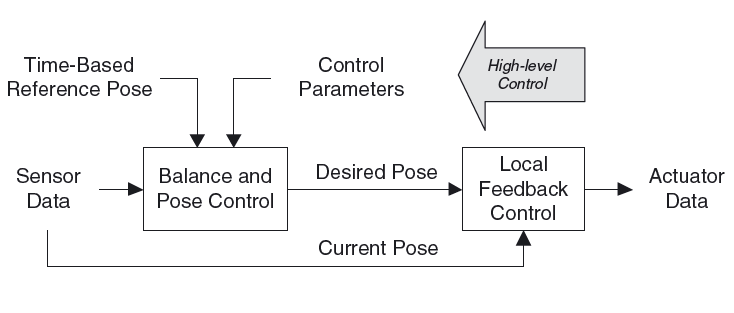
\includegraphics[scale=0.4]{joint_space_motion_control.png}
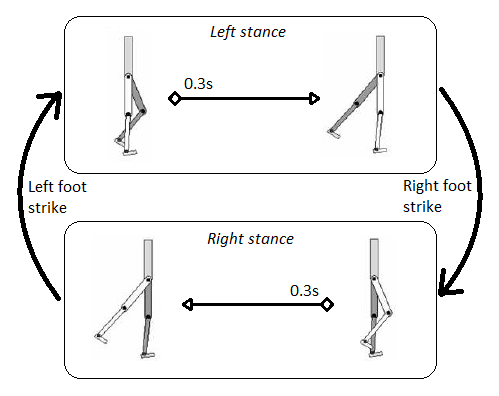
\includegraphics[scale=0.5]{state_machine.png}
\caption{A gauche, exemple de contrôleur dans l'espace des articulations \cite{geijtenbeek2012interactive}. A droite, exemple de machine à état pour la marche \cite{yin2007simbicon}}
\label{fig:joint_space_motion_control}
\label{fig:state_machine}
\end{figure}



Bien qu'il existe plusieurs méthodes permettant de suivre les poses désirées (antagonist feedback \cite{neff2002modeling}, non-linear force field \cite{mussa1997nonlinear}), la méthode la plus commune est le "proportionnal-derivative control" (PD-control). Un PD-contrôleur calcule un moment  \(\tau\) pour chaque articulation proportionnel à la différence entre l'état actuel et l'état désiré. Il prend en compte non seulement la différence entre les angles mais aussi la différence entre les vitesses angulaires. 
\begin{equation}
\tau=k_p(\theta_d - \theta) + k_v(\dot{\theta_d} - \dot{\theta})
\label{eq:pd_controler}
\end{equation}
Avec \(\theta_d\) et \(\dot{\theta_d}\) l'angle et la vitesse désirée, \(\theta\) et \(\dot{\theta}\) l'angle et la vitesse courante et \(k_p\) et \(k_v\) des constantes de vitesse et de position appelées les gains du PD-contrôleur.
Parmi les systèmes basés sur un PD-contrôleur on trouve notamment le SIMBICON (SIMple BIped CONtroler) \cite{yin2007simbicon}. Ce système est basé sur une machine à état fini. Chaque état est défini par une série de poses clefs qui définissent les poses désirées au cours du mouvement. La transition d'un état à un autre peut s'effectuer après un certain temps ou bien lors d'un nouveau contact entre un pied et le sol. La figure \ref{fig:state_machine} (droite) illustre la composition d'un contrôleur SIMBICON pour la marche. La spécification des poses clefs des états possèdent quelques spécificités propres au SIMBICON. Les angles des articulations sont exprimés dans un repère local à l'exception de l'articulation entre le bassin et le dos et de celle de la hanche en phase de vol. Enfin la hanche d'appui ne possède pas de positions cibles. Le moment \(\tau_b \) à appliquer à la hanche d'appui est calculé de manière à ce que le moment total sur le pelvis corresponde au moment \(\tau \) permettant d'obtenir l'orientation définie par l'utilisateur. Ce moment \(\tau \) désiré est déterminé par le PD-contrôleur en prenant pour angle cible la somme de l'angle défini dans la trajectoire du pelvis plus l'angle de direction du mouvement (figure \ref{fig:torques_pelvis}).
\[
\tau_b=\tau - \tau_a - \tau_{torso}
\]
Avec \(\tau_a \) le moment appliqué sur la hanche de balance et \(\tau_{torso} \) le moment appliqué à l'articulation entre le pelvis et le torse.

\begin{figure}[h]
\centering
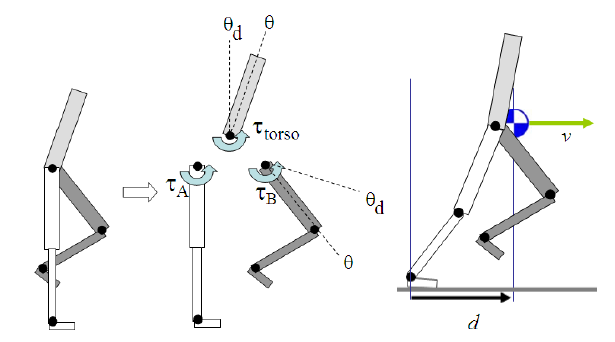
\includegraphics[scale=0.5]{stance_torque_and_v_and_d.png}
\caption{A gauche, calcul des moments sur le pelvis \cite{yin2007simbicon}. A droite, représentation des variables \(d\) et \(v\) \cite{yin2007simbicon}.}
\label{fig:torques_pelvis}
\label{fig:d_and_v}
\end{figure}

\label{sec:jacob}


Le défaut du PD-contrôleur est qu'il est nécessaire de connaitre les bonnes valeurs pour les gains si l'on veut obtenir un résultat correct. Des gains trop bas ne permettraient pas de suivre le mouvement définit. Des gains trop élevés provoqueraient un mouvement saccadé et des possibles oscillations autour de la position désirée. On peut déterminer les paramètres optimaux pour une configuration (mouvement, géométrie du personnage, interaction avec l'environnement, ...) par une série d'essais successifs mais le contrôleur obtenu ne serait pas robuste aux variations de configuration et entrainerait des déséquilibres. Pour pallier ce problème SIMBICON utilise un système de feedforward \cite{yin2007simbicon} qui permet d'apprendre une partie des moments nécessaires. Les PD-contrôleurs n'étant plus utilisés pour les calculs, des gains bas sont suffisant. 
L'extension du SIMBICON proposé par \cite{coros2010generalized} présente un système de compensation de gravité permettant également de calculer une partie des moments nécessaires. Le principe est de calculer pour chaque partie du personnage une force virtuelle compensant la gravité. Donc pour chaque membre du personnage une force virtuelle \(F_{GC}=-mg\) est appliquée au centre des masses, le signe négatif indiquant une force vers le haut. Cette force est ensuite convertie en moment pour chaque articulation se trouvant dans la chaine reliant le point d'application de la force et le pelvis \(\tau=J_i^T F\); où \(J_i ^T\) est la transposée de la jacobienne de la chaine reliant le pelvis et le point d'application de la force. La figure \ref{fig:jacob} (droite) illustre la chaine affectée par la compensation de gravité d'un bras.
La jacobienne d'une chaine de \(k\) articulations contient les informations indiquant l'impact d'une rotation de chaque degré de liberté de la chaine sur la position du point d'application de la force. Chaque $J_i ^T(p)$ peut être calculé par le produit vectoriel entre l'axe de la rotation $\alpha_i$ et le vecteur allant de l'articulation \(i\) au point d'application $p$.
\[
J_i ^T (p)=\begin{bmatrix}
\frac{\partial p_x}{\partial \alpha_i} & \frac{\partial p_y}{\partial \alpha_i} & \frac{\partial p_z}{\partial \alpha_i} \\
\end{bmatrix}
= (\alpha_i \times (p-p_i))^T
\]
Donc la force à appliquer à chaque articulation i correspond à:
\[
\tau = (\alpha_i \times (p-p_i))^T F
\]
Cette méthode de compensation de gravité est appliquée à tous les membres du squelette excepté ceux composant la jambe d'appui.

\begin{figure}[h]
\centering
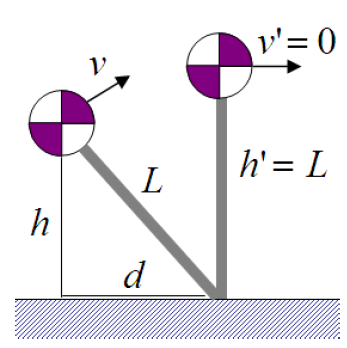
\includegraphics[scale=0.5]{IPM.png}
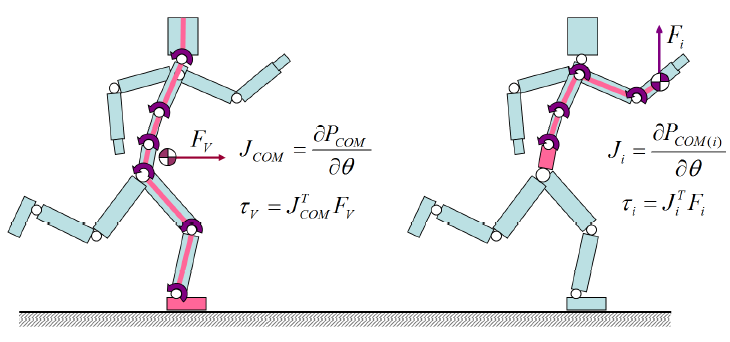
\includegraphics[scale=0.5]{shema_jacobians.png}
\caption{A gauche, modèle du pendule inversé. Au centre jacobienne utilisée pour le contrôle de vitesse. A droite, jacobienne utilisée pour la compensation de gravité. \cite{coros2010generalized} }
\label{fig:ipm}
\label{fig:jacob}
\end{figure}

\subsection{Maîtrise de l'équilibre au cours de la marche}

Un système utilisant uniquement les mécanismes décrits ci-dessus ne permet d'effectuer un mouvement que pour une configuration précise. Toute perturbation, même minime, peut provoquer une perte d'équilibre du personnage.

Pour pallier ce problème le SIMBICON ajoute un système de balance feedback sur la hanche en phase de vol et le pied d'appui. Le principe est de modifier les angles cibles en fonction de la vitesse $v$ du centre des masses du personnage et de la distance \(d\) séparant celui-ci et le pied d'appui (voir figure \ref{fig:d_and_v} droite). 
\[
\theta_d=\theta_{d0} + c_d*d + c_v*v 
\]
Avec \(\theta_d\) l'angle qui sera utilisé par le PD-contrôleur et \(\theta_{d0}\) l'angle spécifié par l'utilisateur.
Les gains \(c_d\) et \(c_v\) sont déterminés pendant la phase d'optimisation hors-ligne. Il est important de signaler que la nécessité d'avoir des gains optimaux rend ce système de feedback très peu flexible.


Parmi les autres systèmes de placement intelligent du pied on trouve l'utilisation d'un modèle du pendule inversé (IPM) \cite{coros2010generalized,kajita20013d}. L'avantage majeur de l'IPM est qu'il est totalement autonome et ne nécessite pas de configuration manuelle ou d'optimisation offrant ainsi une grande robustesse aux perturbations. Le principe de l'IPM est de partir du constat que la somme de l'énergie potentielle de pesanteur et de l'énergie cinétique reste constante peu importe la position du pendule  $\frac{1}{2}mv^2+mgh=\frac{1}{2}mv'^2+mgh'$ (figure \ref{fig:ipm} (gauche)). La supposition d'une vitesse nulle lors de la position d'équilibre (position verticale) et une longueur de jambe $L$ constante nous permettent de simplifier l'équation avec les variables suivantes \(v'=0\) et \(h'=L=\sqrt{h^2+d^2}\). On peut ainsi déterminer la position \(d\) du prochain posé de pied nous permettant d'obtenir un état d'équilibre.
\[
d=v\sqrt{\frac{h}{g}+\frac{v^2}{4g^2}}
\]
Selon la vitesse du personnage il est possible que l'IPM nous donne des résultats impossible à atteindre c'est pourquoi la longueur des pas est limitée à \(d=0.6L\).
Pour permettre d'avoir un résultat conservant une vitesse proche de la vitesse désirée \(V_d\) une altération $\delta$ des résultats de l'IPM est réalisée en utilisant la loi suivante \(\Delta=\alpha V_d\), $\alpha$ étant une constante négative. Ainsi une vitesse positive apporte une diminution de la longueur des pas provoquant une accélération du personnage et inversement une vitesse négative ralentit le personnage.
La position effective du pied est calculée à l'aide d'une interpolation d'ordre 2 entre la position de départ du pied et la valeur retournée par l'IPM. La hauteur du pied au cours du pas est définie par l'utilisateur à l'aide d'une trajectoire. Les angles désirés pour la hanche et le genou sont ensuite déterminés à l'aide de la cinématique inversé. Il reste un degré de liberté définissant l'inclinaison de la jambe qui peut être contrôlé par l'utilisateur.

En plus de permettre l'équilibre l'IPM possède l'avantage de pouvoir complètement définir le mouvement de la jambe en phase de vol pour la marche humaine en utilisant des paramètres plus haut niveau tel que la hauteur des pas et la vitesse désirée. Un avantage majeur d'un tel système est que l'on obtient une définition indépendante des caractéristiques physiques du squelette offrant ainsi une grande flexibilité. Cependant, bien que l'IPM soit très performant, son utilisation limite le déplacement à de la marche car il suppose un contact permanent avec le sol. De plus, l'utilisation d'un IPM pour générer le mouvement complet de la jambe en phase de vol limite grandement les styles de déplacement possibles. En effet il est impossible de déplacer le pied verticalement sans le déplacer dans le plan horizontal.

\subsection{Contrôle de la vitesse}
Parmi les paramètres de haut niveau primordiaux disponibles à l'utilisateur on trouve la vitesse. Dans la version originale du SIMBICON le respect d'une vitesse désirée est obtenu à l'aide d'une stratégie d'évolution. Le principe est de faire varier les poses clefs jusqu'à ce que l'on obtienne un mouvement avec la vitesse voulue. Le défaut est que non seulement il est nécessaire de trouver les poses clefs pour chaque vitesse désirée mais il est également impossible de faire varier la vitesse sans arrêter la simulation. Une amélioration du contrôleur \cite{coros2009robust} apporte la possibilité d'avoir plusieurs états. Le principe est d'avoir des états généraux (i.e. marche avant, marche arrière, …) et de faire des combinaisons de ces états pour obtenir des états intermédiaires. Cela permet de changer de vitesse sans avoir à arrêter la simulation et diminue le nombre de poses clefs nécessaires pour obtenir de multiples vitesses. Cependant, ce système n'assure qu'un suivit peu précis de la vitesse désirée si l'on s'éloigne des états définis.
Plus récemment, une méthode se servant d'une force virtuelle horizontale pour accélérer ou ralentir le personnage a été présentée \cite{coros2010generalized}. Le principe est d'appliquer une force virtuelle sur le centre des masses du personnage pour créer une déséquilibre vers l'avant ou vers l'arrière permettant de contrôler la vitesse du personnage. L'intensité de la force à appliquer est calculée à l'aide d'un PD-contrôleur se basant sur la différence entre la vitesse courante du personnage et la vitesse désirée. Les torques à appliquer aux articulations sont ensuite calculés à l'aide de la méthode de la transposée jacobienne.  La chaine de membres articulée considérée pour l'application de la force est la chaine reliant la tête au pied d'appui (voir figure \ref{fig:jacob} (centre)). Ce système permet d'avoir un contrôle fin de la vitesse. Cette méthode de contrôle a été utilisée de manière intensive dans le but de conserver l'équilibre dans une position statique \cite{geijtenbeek2012simple}. Cependant, ce système ne permet pas de suivre correctement les vitesses si les gains du contrôleur ne sont pas adaptés à la configuration. Par exemple des gains adaptés pour un déplacement à l'air libre deviendraient inefficaces pour un déplacement dans un milieu liquide. De plus l'utilisation d'une force virtuelle est limitée par les valeurs maximales des moments aux articulations. Ce qui veux dire que si l'on a besoin d'une force virtuelle élevée, cette stratégie de contrôle devient invalide.

\subsection{Déplacement en milieu aquatique}
\subsubsection{Contrôle du mouvement en milieu aquatique}
La simulation d'interactions entre un personnage et un milieu liquide a déjà été étudiée. La plupart des travaux placent le personnage en milieu aquatique \cite{yang2004layered,kwatra2010fluid,tan2011articulated,si2014realistic}. Cependant ces contrôleurs sont utilisés pour simuler de la nage et non de la marche. On trouve également des approches utilisant un fluide pour simuler l'effet du vent sur la marche d'un personnage \cite{lentine2011creature}. Cependant ces articles immergent complètement le personnage dans le fluide. De plus dans ce genre de situation l'effet de la poussée d'Archimède est ignoré car il est trop faible dans de l'air.

De nombreuses approches se servent d'un modèle basé sur les équations de Navier Stokes \cite{stam1999stable} avec une représentation Eulérienne \cite{si2014realistic} pour réaliser la simulation de l'eau. Le défaut est que cette méthode ne permet pas une simulation en temps réel car trop couteuse en temps de calcul. D'autres approches se contentent de modéliser l'eau à travers des forces externes simulant l'impact du fluide sur le personnage calculées à l'aide d'équations simples représentant les phénomènes de bases tels que l'opposition du liquide, la poussée d'Archimède et la friction du liquide \cite{yang2004layered}. Cette solution permet de réaliser la simulation en temps réel mais rend impossible la prise en compte des perturbations du liquide provoquées par le personnage.

\subsubsection{Biomécanique de la marche en milieu aquatique}
La marche en milieu aquatique a été le sujet de plusieurs études dans le milieu de la biomécanique \cite{barela2006biomechanical,chevutschi2009comparison,orselli2011joint,miyoshi2005functional}. Certains de ces travaux présentent les différences provoquées par la présence de l'eau \cite{barela2006biomechanical}. Cependant, ces travaux utilisent des niveaux d'eau se situant au-dessus du milieu du torse (au niveau du processus xiphoïde). C’est à dire que l'impact de l'eau sur le torse est toujours présent ce qui modifie fortement les résultats par rapport à notre situation où la hauteur de liquide maximale est au niveau de la taille. En effet, le torse ayant une très grande surface le mouvement est extrêmement ralentit si il est plongé dans le fluide. De plus le volume du torse étant élevé la poussée d'Archimède a une importance bien plus grande dans ces études que dans notre cas. 

%%%%%%%%%%%%%%%%%%%%%%%%%%%%%%%%%%%%%%%%%%%%%%%%
%%%%%%%%%%%%%%%%%%%%%%%%%%%%%%%%%%%%%%%%%%%%%%%% 
\section{Contributions}
\label{sec:overview}


\begin{figure}[h]
\centering
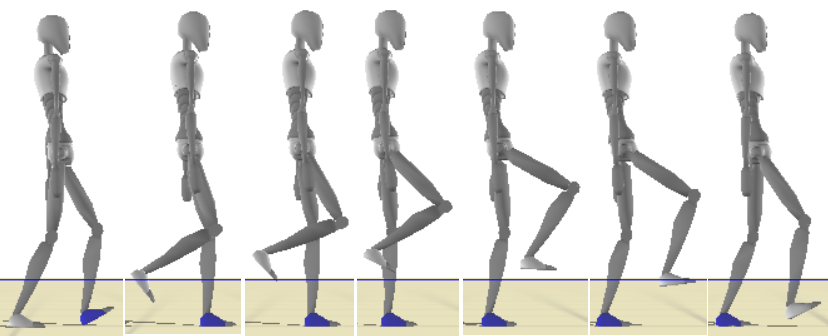
\includegraphics[scale=0.6]{strips/min_drag_25cm.png}
\caption{Marche d'un personnage cherchant à minimiser les forces de résistance de l'eau dans 25cm de liquide. La ligne bleu représente le niveau d'eau.}
\label{fig:min_drag_25}
\end{figure}


La contrôle de la marche en milieu liquide n'a donc peu été l'objet de travaux dans le domaine de l'animation.  Des travaux aient été réalisés dans le domaine de la biomécanique ne considérant que des cas où l'immersion dépasse le milieu du torse. En animation, l'utilisation actuelle des systèmes de maintien de l'équilibre limite fortement la capacité à simuler des mouvements variés ce qui empêche l'émergence de mouvements appropriés au déplacement en milieu liquide. D'autre part, les systèmes de contrôle de la vitesse exposés dans notre état de l'art présentent tous  le défaut de ne pas assurer le suivi correct de la vitesse désirée si l'on s'éloigne des conditions pour lesquels ils ont été optimisés. Enfin, les contrôleurs basé physique implémentant l'interaction avec un fluide ne proposent pas un modèle permettant l'animation d'un modèle humain en temps réel.

Nous proposons un contrôleur répondant à ces manques grâce à trois contributions. La première contribution est un modèle aquatique permettant de simuler l'influence du liquide sur le déplacement du personnage. La deuxième contribution est un système permettant de combiner plusieurs états nous permettant d'adapter les poses clefs utilisées en fonction de l'environnement et des paramètres spécifiés par l'utilisateur. Notre contrôleur démontre une grande liberté de spécification de mouvement grâce à une nouvelle gestion de la perte d'équilibre. Enfin, nous améliorons les systèmes utilisant une force virtuelle et modifiant les résultats de l'IPM à l'aide d'un système d'apprentissage autonome permettant ainsi un suivi exact et robuste de la vitesse désirée. 


\begin{figure}[h]
\centering
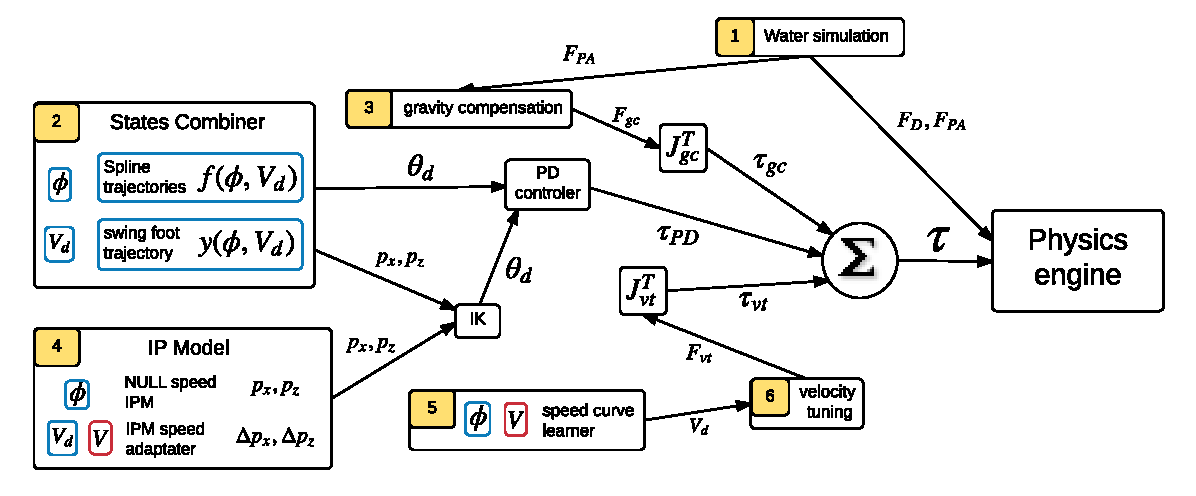
\includegraphics[scale=0.6]{general_process.pdf}
\caption{schéma récapitulatif de notre contrôleur}
\label{fig:shema_controler}
\end{figure}

\subsection{Vue globale du système}
%


Notre système de contrôle du mouvement est composé de 6 blocs principaux (figure \ref{fig:shema_controler}). Voici une vision globale du fonctionnement du système. 

Nous commençons par calculer les forces résultant de l'influence du fluide sur le personnage. Notre modélisation utilise des formules simples (résistance de l'eau, poussée d'Archimède) nous permettant d'obtenir une simulation en temps réel (voir section \ref{sec:model_fluide}).

Chaque articulation possède une trajectoire spécifiant les angles à suivre au cours du déplacement. Ces trajectoires sont déterminées à partir de poses clefs définis par l'utilisateur. Les valeurs intermédiaires sont déterminées à l'aide de splines Catmull-Rom. Les trajectoires des articulations de la jambe de balance sont déterminées dynamiquement à partir de la trajectoire désirée pour le pied en phase de vol. La trajectoire du pied en phase de vol est soit spécifiée par l'utilisateur soit déterminée par les systèmes de conservations de l'équilibre lorsque le personnage est dans la phase de descente du pas ou qu'il est en déséquilibre (voir section \ref{sec:IPM}).

Le système de combinaison d'états permet à l'utilisateur de spécifier plusieurs trajectoires pour une articulation chacune d'entre elles étant associée à une vitesse. Le système combinera plusieurs de ces trajectoires pour obtenir un résultat plus adapté à la vitesse désirée. Ce système est particulièrement utile pour les articulations possédant des comportements très différents suivant la vitesse désirée. Les angles lus depuis les trajectoires sont ensuite utilisés par le PD-contrôleur pour calculer les moments à appliquer aux articulations au cours du déplacement (voir section \ref{sec:multi_state}).

Nous utilisons un système de compensation de gravité similaire à celui proposé par \cite{coros2010generalized} modifié pour prendre en compte la présence du fluide. Ce système permet de calculer une partie des moments nécessaires au mouvement ce qui nous autorise à utiliser des gains moins élevés dans le PD-contrôleur. L'utilisation de gains faibles est importante pour éviter d'obtenir des oscillations autour de la position désirée et obtenir un résultat s'adaptant plus facilement aux variations de l'environnement (voir section \ref{sec:grav_comp}).

Le maintien de l'équilibre est obtenu par un placement du pied intelligent obtenu à l'aide d'un modèle de pendule inversé (IPM). Pour permettre l'observation d'un plus grand nombre de styles de marche possible, nous utilisons l'IPM seulement lorsque le personnage est dans la phase de descente d'un pas ou lorsque nous détectons une perte de l'équilibre. Pour aider ce système, nous avons implémenté pour  la cheville d'appui le modèle de feedback présenté par \cite{yin2007simbicon} corrigeant la position du personnage (voir section \ref{sec:IPM}).

Le contrôle de la vitesse est obtenu à l'aide d'une force virtuelle similaire à celle utilisée par \cite{coros2010generalized}. Ce système a été amélioré pour prendre en compte les variations de vitesse au cours d'un pas. Cette modification nous permet d'obtenir un résultat correspondant plus à la spécification de l'utilisateur. Ce système est aidé par une altération des résultats de l'IPM permettant d'accélérer ou de ralentir le personnage. Ces deux systèmes sont contrôlés par une méthode d'apprentissage et ne nécessitent aucun paramétrage de la part de l'utilisateur. (voir section \ref{sec:speed_control})

%
\section{Modèle physique}
\label{sec:model_physique}

\subsection{Modélisation du personnage}
%
\begin{figure}[h]
\centering
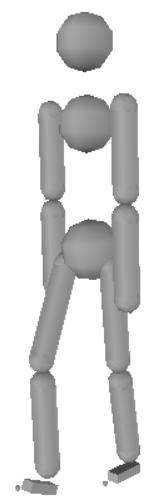
\includegraphics[scale=0.4]{colli_primitives.png}
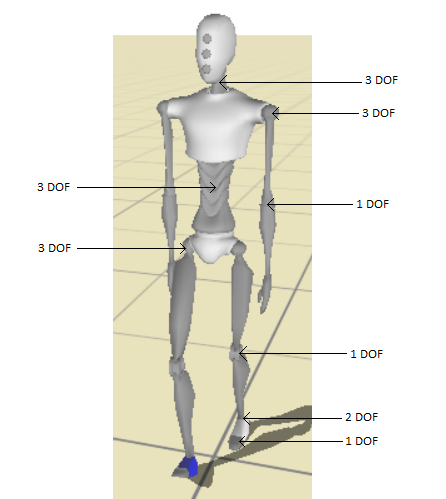
\includegraphics[scale=0.4]{img_dof.png}
\caption{A gauche, le modèle physique du personnage. A droite, degrés de liberté internes}
\label{fig:colli_primitives}
\label{fig:dof}
\end{figure}

Le personnage utilisé est composé de corps solides simples (visible figure \ref{fig:colli_primitives} centre). La tête, le torse, le pelvis et les orteils sont représentés par des sphères. Les bras et les jambes sont représentées par des capsules (cylindre avec des demi-sphères aux extrémités). Les pieds sont modélisés avec des prismes droits. Le squelette est composé de 28 degrés de liberté internes présentés dans la figure \ref{fig:dof} droite plus 6 degrés de liberté externes (position et orientation). Il est intéressant de noter que le poids de chaque membre est modélisé par une valeur et un point d'application qui ne se trouve pas forcément au centre du solide de collision.

%
\subsection{Modélisation des fluides}
%
\label{sec:model_fluide}
Lorsque l'on déplace un corps solide à l'intérieur d'un fluide, ce dernier applique trois réactions principales sur le solide. La première est une force de résistance du fluide qui est produite par le déplacement du fluide fluide se trouvant sur la trajectoire du solide. La seconde est une force de friction entre le fluide et le solide. Ces deux réactions du fluide ont pour effet d'entraver le déplacement du solide. La dernière est la poussée d'Archimède, provenant des différences de pression sur la surface du solide, et a pour effet de repousser le solide vers la surface.
Plutôt que de réaliser une modélisation réaliste du fluide (à l'aide des équation de Navier-Stokes par exemple), nous allons baser notre modèle sur la définition d'une hauteur de liquide et les formules de base de dynamique des fluides pour représenter l'influence du liquide sur le personnage. Notre modèle ne considère pas les perturbations du fluide provoquées par le déplacement du personnage. Cette modélisation a l'avantage d'être beaucoup moins couteuse en puissance de calcul ce qui nous permet de conserver une exécution en temps réel tout en permettant une simulation réaliste.
%
\subsubsection{Forces hydrodynamiques}
%
La résistance du fluide est calculée à partir de la formule suivante:
\[
F_D=\frac{1}{2} \rho v^2 A_n C_d
\]


Avec \(C_d\) le coefficient de résistance, \(\rho\) la densité du fluide, \(A_n\) la surface en vue du membre du personnage et \(v\) la vitesse de ce membre. Les surfaces et les vitesses sont calculées à partir de la représentation physique du personnage. La vitesse n'étant pas constante en tout point d'un membre, nous utilisons un découpage en éléments finis de la surface de la représentation physique de chaque membre pour effectuer nos calculs. La surface en vue $A_n$ de chaque élément de surface est calculée en projetant la surface de l'élément dans un plan orthogonal à la vitesse $v$. 

La force finale $F$ à appliquer à chaque élément est calculée en ajoutant la viscosité du fluide à l'aide d'un coefficient de viscosité $\mu$ 
\[
F=F_D*\mu
\]
Le coefficient de viscosité est obtenu en normalisant la viscosité du fluide par celle de l'eau ($1,00 \times 10^{-3} Pa.s$).
%
\subsubsection{Poussée d'Archimède}
%
La poussée d'Archimède $F_{PA}$ est calculée à l'aide de la formule suivante:
\[
F_{PA}=-V_i \rho g
\]
Le volume immergé \(V_i\) est calculé à l'aide du volume immergé des représentations physiques des différents membres du personnage.  Pour les sphères et les cylindres (jambes et orteils) le volume immergé est calculé en utilisant les formules de géométrie existantes (cylinrical wedge, cylindrical segment). Pour les prismes droits (pieds) nous découpons le volume en voxels et faisons la somme des volumes des voxels dont le centre se trouve en dessous du niveau de l'eau.
%
\section{Contrôle du mouvement}
\label{sec:controler}
%
Notre système se base sur la version du SIMBICON présentée par \cite{coros2010generalized}. Les angles des trajectoires pour les chevilles, le pelvis, le dos et la tête sont spécifiées dans le repère du personnage. Ce repère est équivalant au repère du monde à la différence qu'il est orienté de manière à ce que l'axe z corresponde à la direction que face le personnage. Les angles des trajectoires pour les épaules, les coudes, le genou de la jambe d'appui et les orteils sont spécifiés dans le repère local aux articulations.

Contrairement à \cite{coros2010generalized} nous permettons la spécification manuelle du pied en phase de vol pour permettre l'observation d'un plus grand nombre de styles de déplacements et en particulier pour permettre une sortie rapide de l'eau de la jambe de vol. La spécification manuelle est utilisée lors de la phase ascendante d'un pas si le personnage n'est pas en déséquilibre. Cette spécification s'effectue dans le repère local de la hanche en phase de vol.

%
\subsection{Combineur d'état}
\label{sec:multi_state}
%
Suivant la vitesse désirée il est possible que les trajectoires nécessaires pour obtenir un résultat optimal soit radicalement différentes. Par exemple, étudions rapidement le cas de la cheville d'appui. Lorsque le personnage marche vers l'avant il est nécessaire que celui-ci pose le talon en premier. Une fois que le pied est à plat au sol il est nécessaire de conserver une différence entre les forces appliquées sur l'avant du pied et celles appliquées sur l'arrière du pied pour faire pencher le personnage vers l'avant. Au contraire, pour une marche sur place ou vers l'arrière, il sera nécessaire que celui-ci pose la pointe du pied en premier puis maintienne une différence des forces le faisant pencher vers l'arrière. Chaque type de déplacement (marche vers l'avant, vers l'arrière, sur place, ...) possèdent des caractéristiques spécifiques rendant plus facile le mouvement associé. C'est pourquoi nous utilisons un système permettant la définition de plusieurs trajectoires pour les articulations sur lesquelles nous observons ce type de phénomène. Notre système est similaire à celui présenté par \cite{coros2009robust}. Notre système se différencie par deux caractéristiques. Premièrement, contrairement à \cite{coros2009robust} nous n'utilisons pas notre système pour tenter de trouver un état stable en combinant plusieurs états de base. Notre système a pour but de créer une base plus adaptée au suivi de la vitesse désirée. La stabilité étant assurée par l'IPM, le combineur d'états ne cherche pas absolument à produire un état assurant la stabilité par lui-même. La seconde différence est que \cite{coros2009robust} spécifie des états complets (i.e. marche avant, marche arrière, ....). Notre système se contente de capturer les différences ayant une influence importante sur la vitesse. C'est pourquoi nous spécifions plusieurs trajectoires seulement pour les articulations pour lesquelles nous observons des différences importantes suivant la vitesse. De plus notre système a été conçu pour permettre d'utiliser la même trajectoire pour plusieurs vitesses. Nous avons déterminé que les trajectoires possédant des différences significatives sont celles des chevilles, du pelvis, du pied en phase de vol et celle de l'articulation entre le pelvis et le torse (dans une moindre mesure). 

Nous allons maintenant expliquer le fonctionnement du combineur d'états plus en détail. Pour chaque articulation où système (e.g. pied en phase de vol) possédant plusieurs trajectoires, le combineur d'états va chercher les deux trajectoires associées aux deux vitesses les plus proches de la vitesse désirée. Si la vitesse désirée est inférieure (resp. supérieure) à la vitesse la plus basse (resp. plus haute) spécifiée, le système utilisera directement la trajectoire correspondant à la vitesse la plus basse (resp. haute) comme si il n'y avait qu'une trajectoire définie. Si le système trouve bien deux trajectoires encadrant la vitesse désirée, il créé une nouvelle trajectoire contenant $k$ points clefs répartis de manière uniforme. Lors de nos tests nous avons déterminé qu'un nombre de $k=10$ points clefs était suffisant. Le combineur d'états attribue ensuite des valeurs à chacun de ces points en utilisant une combinaison des valeurs contenues dans les deux trajectoires considérées suivant une loi d'ordre 2:
$$
f(\phi)=f_1(\phi)*\frac{(V_d-V_1)^2}{(V_d-V_1)^2+(V_d-V_2)^2}+f_2(\phi)*\frac{(V_d-V_2)^2}{(V_d-V_1)^2+(V_d-V_2)^2}
$$
Avec $f$ la trajectoire finale,$(f_1,V_1)$ et $(f_2,V_2)$ les deux trajectoires les plus proches de la vitesse désirée.
% 
\subsection{Compensateur de gravité}
\label{sec:grav_comp}
Notre système de compensation de gravité se base sur celui présenté par \cite{coros2010generalized}.Nous avons modifié ce système pour permettre la prise en compte d'un milieu liquide. En effet, du fait de la poussée d'Archimède le poids à supporter par le personnage est moins grand lorsqu'il est plongé dans un fluide. De ce fait au lieu de compenser le poids réel de chaque membre du personnage, il faut compenser le poids effectif (poids observable dans le fluide). Notre modification consiste donc à calculer la force résultant de la poussée d'Archimède sur chaque membre du personnage et de soustraire celle-ci à la force virtuelle à appliquer. Il parait intéressant de noter qu'il ne suffit pas simplement de diminuer l'intensité de la force à appliquer. En effet suivant la modélisation des membres du personnage, il est fréquent que la densité soit variable à l'intérieur de ceux-ci. Par exemple, dans notre modélisation seul les bras possèdent une densité uniforme. De ce fait le point d'application de la force  $F_{gc}$ compensant la gravité et celui de la force $F_{PA}$ causée par la poussée d'Archimède seront différent, ce qui nous oblige à déterminer le point d'application de la force finale $F$:
$$
F=F_{gc}- F_{PA}
$$

Si le milieu est assez dense il est fortement possible que les membres du personnage disposant d'une densité faible aient un poids plus faible que la force causée par la poussée d'Archimède. Dans ce cas le système génère des moments ayant pour effet de baisser les membres du personnage au lieu de les lever. Nous ne traitons pas ce cas comme un cas particulier. En effet, comme dit précédemment le but du compensateur de gravité est de calculer une partie des moments nécessaires pour pouvoir se rapprocher de la position désirée. Or si nous avons une poussée d'Archimède plus forte que le poids des membres du personnage, ceux-ci essaierons de flotter ce qui entraverait le déplacement du personnage. Il est donc intéressant de conserver le système présenté ci-dessus même dans ce cas particulier car il aidera tout de même le personnage à suivre les poses désirées.
%.
\subsection{Conservation de l'équilibre}
%
L'équilibre du personnage est obtenu par le placement intelligent du pied à l'aide d'un modèle de pendule inversé (IPM) et de fonctions de feedback sur certaines articulations (balance feedback). Les systèmes de contrôle de vitesse (section \ref{sec:speed_control}) permettent également un maintien de l'équilibre du fait qu'ils maintiennent le système autour d'une vitesse stable. 
%
\subsubsection{Modèle du pendule inversé}
%
\label{sec:IPM}
L'utilisation d'un IPM permet d'avoir un système efficace de conservation d'équilibre ne nécessitant pas de paramétrage de l'utilisateur. Dans le cadre de notre  projet nous utiliserons un IPM similaire à celui présenté par \cite{coros2010generalized}. Le système utilise un IPM supposant une position nulle à la position verticale et une longueur de jambe constante. 


Bien que l'IPM soit intéressant il limite les possibilités de mouvement. Par exemple il rend impossible un mouvement définissant une trajectoire rectangulaire pour le pied comme l'on voit sur la figure \ref{fig:min_drag_25}. Ce genre de déplacement est important dans le cadre de notre étude car elles sont typiques d'environnement ou le mouvement est beaucoup entravé (par exemple de la neige). Pour permettre l'observation de tels déplacements nous avons rajouté la possibilité de manuellement définir la position du pied au cours du pas. Cette définition manuelle est considérée temps que le personnage est dans la phase ascendante du pas \(V_{COM}(y)>0\) et qu'il n'est pas dans un état instable. Nous déterminons une instabilité du personnage si nous détectons une variation irrégulière du motif de vitesse observé au cours d'un pas (voir la section \ref{sec:speed_virt_force}). Si un état instable est détecté nous utilisons le résultat de l'IPM pour la totalité du pas jusqu'à ce que nous retournions dans un état stable.
%

%
\subsection{Contrôle de vitesse}
%
\label{sec:speed_control}
Dans le cadre de ce projet, la capacité à marcher à une vitesse donnée est un critère primordial. De plus nous souhaitons obtenir un système qui sera robuste à la variation du milieu. C'est à dire que nous souhaitons que notre contrôler soit capable de marcher dans un mètre d'eau ou dans 50cm d'huile aussi bien que lorsqu'il ne se trouve pas en présence d'un fluide. Pour obtenir un tel résultat, nous utilisons une force virtuelle ainsi qu'un système d'altération des résultats de l'IPM.
%
\subsubsection{Contrôle de vitesse par force virtuelle}
%
\label{sec:speed_virt_force}

Pour obtenir une vitesse désirée nous allons appliquer une force virtuelle horizontale qui accélèrera ou ralentira le personnage en déplaçant le centre des masses. De manière similaire à \cite{coros2010generalized} nous utilisons un PD-contrôleur utilisant l'écart entre la vitesse désirée et la vitesse actuelle du personnage pour calculer la force virtuelle nécessaire.
Cependant la chaine de membres du personnage considérés pour l'application de la force est la chaine reliant le torse au pied d'appui (donc ne prend pas en compte la tête du personnage). La raison de ce choix est qu'il ne parait pas naturel de pencher la tête si l'on veut aller dans une direction. Les valeurs utilisées pour la jacobienne sont différentes de celles utilisées par \cite{coros2010generalized}. Nous utilisons la somme des vecteurs séparant les articulations pondérés par le poids du membre présent entre ces deux articulations.
\[
J_n ^T (p)=\frac{1}{M}\sum_{\substack{0<i\leq n}} ((P_i(x,y,z)-P_{i-1}(x,y,z))*M_i)
\]
Avec \(M\) la somme des poids de tous les membres considérés par le système et \(P_i(x,y,z)\) la position de l'articulation \(i\) de la chaine, \(P_0(x,y,z)\) étant le point d'application de la force. Cela évite que les articulations du bas du corps reçoivent une grande importance du fait qu'elles se trouvent loin du torse (qui représente une grande partie de la masse du personnage). Cette caractéristique est intéressante car un moment appliqué sur la cheville ayant pour but de faire pencher le torse aurait de grande chance de se faire annuler par un moment sur la hanche ou le pelvis ayant pour but de redresser le personnage. De plus il est plus simple de créer un déséquilibre régulier du personnage en appliquant un moment sur l'articulation entre le pelvis et le torse qu'en appliquant un moment sur la cheville ce qui renforce l'idée que le torse doit bien être considéré indépendamment du bas du corps.

Il est facile d'observer que la vitesse de déplacement du centre des masses n'est pas constant au cours d'un pas. De ce fait l'application d'une force virtuelle se basant sur une vitesse désirée constante aura pour effet de faire disparaître ce phénomène, voire demander localement au personnage de ralentir alors que l'on voudrait le voir accélérer de manière globale. C'est pourquoi il serait plus intéressant d'appliquer une force constante au cours d'un pas. Cependant ce genre de force constante serait difficile à déterminer et diminuerait la robustesse du modèle car elle ne pendrait pas en compte les évènements se passant au cours d'un pas (i.e. ralentissements du au contact avec un objet par exemple). On peut observer que lorsque nous sommes dans le cas d'un déplacement stable, la courbe de vitesses observées au cas d'un pas reste constante à chaque pas. L'idée serait donc d'adapter la vitesse désirée que l'on communique au PD-contrôler suivant les variations de vitesse observées au cours du pas. C'est pourquoi nous avons construit un système permettant d'apprendre cette courbe de variations de vitesse de manière à appliquer une force virtuelle plus adaptée. De manière similaire aux trajectoires des articulations, cette courbe est définie comme une fonction de la phase \(\phi\) et possède un nombre de point de référence pouvant être définis par l'utilisateur. Les valeurs entre les points de références sont également déterminées à l'aide de splines Catmull-Rom. Un nombre de 10 points de référence s'est montré être suffisant pour permettre l'obtention d'une courbe précise tout en évitant de surcharger le système. Le système utilise une courbe pour la vitesse suivant l'axe sagittal et deux courbes pour l'axe coronal (une pour chaque phase d'appui). L'axe coronal nécessite deux courbes car dans le cas d'une vitesse non nulle selon l'axe coronal le mouvement observé devient asymétrique.Une autre différence entre les deux axes et que pour l'axe coronal nous stockons directement les vitesses en $m.s^{-1}$ alors que pour l'axe sagittal nous stockons des facteurs multiplicateurs à appliquer à la vitesse désirée par l'utilisateur. L'utilisation des facteurs multiplicateurs nous permet une plus grande aisance à nous adapter aux variations de vitesses demandées par l'utilisateur. En effet pour une variation de vitesse de moyenne amplitude il est fortement possible que la courbe de facteurs multiplicateurs reste identique. Cependant vu que nous travaillons généralement avec une vitesse nulle suivant l'axe coronal, il nous est impossible de nous baser sur un coefficient multiplicateur.

\begin{figure}[h]
\centering
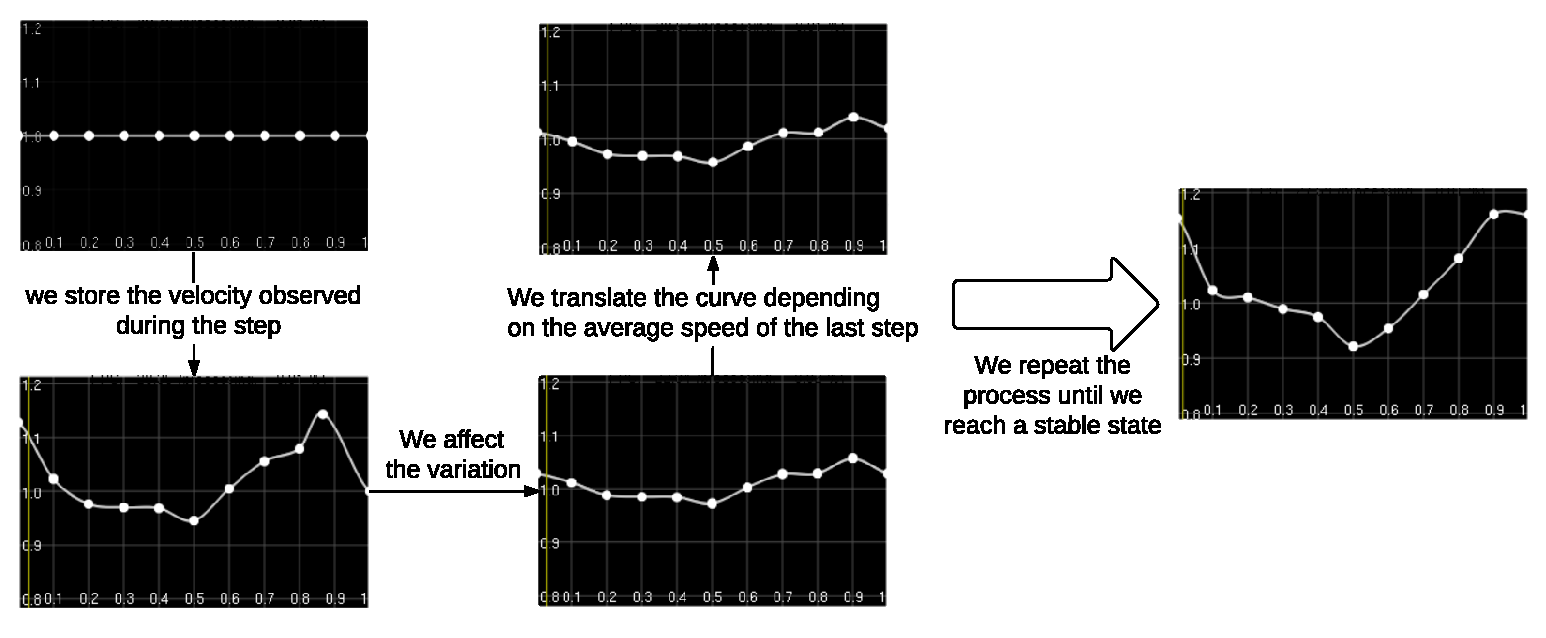
\includegraphics[scale=0.45]{speed_curve_learner.pdf}
\caption{Schéma présentant le processus d'apprentissage de la courbe de vitesse}
\label{fig:speed_curve_learner}
\end{figure}


Ce paragraphe explique de manière plus précise l'apprentissage des courbes de vitesse. Comme présenté sur le schéma \ref{fig:speed_curve_learner} le système d'apprentissage des courbes de vitesse s'effectue par une boucle de 3 étapes répétées jusqu'à l'obtention d'une courbe stable. La première étape est de relever, aux cours d'un pas, la vitesse réellement observée pour chaque point de référence. Une fois le pas terminé nous calculons la variation moyenne entre la courbe que nous avions et la courbe observée. La deuxième étape consiste à, si la variation moyenne observée est inférieur à un seuil, adapter les valeurs stockées pour les rapprocher des valeurs observées. Nos tests ont montré qu'un seuil de 0,4 donne des résultat satisfaisant. Nous notons tout de même qu'il peut être intéressant d'utiliser un seuil plus élevé au début de la phase d'apprentissage car il est possible que la trajectoire initialement utilisée soit très différente de la trajectoire observée.  Pour éviter d'obtenir des oscillations autour de la courbe vers laquelle on cherche à converger, la variation de chaque point est limitée à une variation d'au maximum la valeur de la variation moyenne constatée. Pour finir nous modifions les points de la courbe de façon à ce que la nouvelle courbe nous permette d'obtenir la vitesse moyenne voulue. Pour obtenir ce résultat nous déterminons le ratio entre la vitesse moyenne demandée et la vitesse moyenne observée lors du dernier pas et nous multiplions tous les points de la courbe par ce ratio. Dans le cas de l'axe coronal nous utilisons le ratio entre la vitesse demandée et la moyenne des vitesses observées lors des deux derniers pas.

La présence du seuil nous permet de détecter les variations irrégulières de la courbe de vitesse. Une fois la situation d'équilibre atteinte nous obtenons une courbe stable qui est caractéristique au déplacement observé. Si l'on constate une variation de cette courbe cela veut dire qu'un élément est venu perturber le déplacement. Dans ce cas, nous déclarons au contrôleur que nous ne sommes plus dans un état stable ce qui signale au contrôleur qu'il doit utiliser l'IPM durant toute la durée du pas jusqu'à ce que le mouvement redevienne stable. Une fois le mouvement redevenu stable, c'est à dire que la variation moyenne de la vitesse est redevenue inférieure à l'heuristique, nous recommençons à utiliser le système décrit précédemment pour adapter la courbe de vitesse. Si le système détecte plus de 5 pas consécutif pour lesquels le mouvement est déclaré instable, alors nous réinitialisons tous les points des courbes de vitesses à la valeur de la vitesse désirée spécifiée par l'utilisateur. Cela nous permet de restaurer le système dans le cas où les courbes auraient subit une variation très forte les éloignant trop de la courbe résultant de l'IPM ce qui bloque le système.
%
\subsubsection{Altération des résultats de l'IPM}
\label{sec:ipm_alt}
%
Bien que le système utilisant une force virtuelle pour contrôler la vitesse permette un réglage fin de la vitesse, il ne permet pas d'effectuer de grandes variations de vitesses. En effet, pour réaliser de telles variations nous aurions besoin d'une force virtuelle très importante ce qui aurait des effets indésirables. En effet une force virtuelle élevée provoquerait l'apparition de moments très élevés. Si les moments maximaux aux articulations ont été  paramétrés alors les variations de la force virtuelle n'auront plus d'impact sur le personnage et il serait possible d'observer un mouvement peu naturel si seules certaines articulations de la chaine de membres affectés ont atteint leur maximum. Si les moment maximaux n'ont pas été définis alors une force élevée résulterait en des phénomène non réalistes. Pour régler ce problème \cite{coros2010generalized} propose d'altérer les résultats de l'IPM pour aider à atteindre la vitesse voulue. Cependant, cette modification est basée sur une relation linéaire dépendant de la vitesse désirée. Cette relation linéaire rend le système trop peu efficace notamment pour des mouvements dans un fluide qui ralentira le personnage.

Vu qu'il semble impossible d'utiliser une simple loi dépendant de la vitesse désirée, nous avons décidé d'utiliser un système qui stocke un $\Delta(x,z)$ qui sera ajouté au résultat de l'IPM. Pour pouvoir déterminer la valeur de ce $\Delta$ nous utilisons une méthode incrémentale. \`A la fin de chaque pas nous utilisons un PD-contrôleur se basant sur la différence entre la vitesse désirée et la vitesse réellement observée au cours du pas pour déterminer comment doit évoluer le $\Delta(x,z)$ pour permettre au personnage de se déplacer à la vitesse désirée. Nous n'utilisons ce système que sur l'axe sagittal. Les vitesses demandées sur l'axe coronal étant plus faibles le personnage n'a pas besoin de ce système pour les atteindre.

Ce système de contrôle de vitesse est extrêmement efficace et robuste. Cependant, si l'on utilise un $\Delta(x,z)$ trop élevé dans le but d'accélérer le personnage cela risque d'empêcher l'IPM de maintenir l'équilibre. C'est pourquoi nous avons mis une limite aux valeurs du $\Delta(x,z)$. Nous fixons cette valeur à 0,09m, ce qui correspond à la valeur maximale permettant de conserver l'équilibre avec un personnage immergé jusqu'à la taille dans de l'eau, les autres situations de test supportant des valeurs plus élevées cela parait être une bonne sécurité. 
%

\section{Optimisation hors ligne}
\label{sec:optimisation}
%
Le nombre très important de paramètres que prend le système en entrée rend très difficile la recherche manuelle d'une solution optimale à la simulation stable d'un personnage en interaction avec le liquide.. C'est pourquoi ce travail de recherche est effectué à l'aide d'un système d'optimisation hors ligne. Le principe est d'explorer l'espace des paramètres et conserver la "meilleure solution" trouvée. La notion de "meilleure solution"  est définie à l'aide d'une fonction objectif qui permettra d'évaluer la qualité de chaque ensemble de paramètres. Par exemple, il est possible de calculer la somme des moments appliqués aux articulations durant un certain temps pour obtenir une fonction évaluant l'énergie dépensée par le personnage. L'exploration de l'espace des paramètres peut se faire de manière aléatoire, mais il est plus rapide d'utiliser un algorithme tel que la descente de gradient. L'optimisation hors ligne permet donc d'obtenir un mouvement optimal pour les critères définis dans la fonction d'évaluation. Ce qui veut dire que le mouvement obtenu possèdera des caractéristiques propres à la fonction d'évaluation qui a été utilisée.


Les paramètres que nous optimiserons sont la trajectoire du pied en phase de vol (positions) et les trajectoires angulaires selon l'axe coronal associées aux éléments suivants:
\begin{itemize}
\item{le pelvis (3 points clefs);}
\item{l'articulation du dos (2 points clefs);}
\item{la cheville d'appui (11 points clefs);}
\item{la cheville en phase de vol (11 points clefs);}
\item{le genou d'appui (5 points clefs);}
\end{itemize}
Pour la les positions du pied en phase de vol nous utilisons respectivement 3, 5 et 11 points clefs pour les axes x, y et z. Nous optimisons donc un total de 51 variables.
Nous n'optimisons pas les articulations des bras et du cou de manière à obtenir un modèle à partir duquel un utilisateur peut spécifier des actions utilisant ces membres. Les gains des différents PD-contrôleurs ne sont pas optimisés. Nous utilisons des gains génériques permettant une grande variété de mouvements. Nous utilisons les gains utilisés par \cite{yin2007simbicon} dans le cadre de la marche vers l'avant.

%
\subsection{Fonction objectif}
%
Nous allons construire notre fonction d'optimisation $f_{eval}$ en utilisant d'une part une combinaison pondérée de critères d'évaluation représentant un but physique et d'autre part des heuristiques. Notre fonction d'évaluation se base sur trois critères 
\begin{equation}
f_{eval}=\sum_{\substack{t<k}} (\alpha f_{energ} + \beta f_{acc} + \gamma f_{drag})
\label{eq:simple_objective}
\end{equation}
Avec k le temps en seconde durant lequel nous évaluons le contrôleur.
Chacune des $f_i$ est normalisée par la valeur moyenne obtenue en effectuant une série d'optimisations du système en utilisant uniquement la fonction $f_i$ comme fonction d'évaluation. Les poids $\alpha$, $\beta$, $\gamma$ nous permettent de choisir facilement l'importance qu'aura une composante dans le résultat final. Les critères d'évaluation que nous utilisons sont les suivants:
\begin{itemize}
\item{\textit{Minimisation de l'énergie} ($f_{energ}$). Le but de ce critère est de faire tendre le résultat vers une simulation utilisant le minimum d'énergie dépensé par le personnage. Cela nous permettra d'éviter les mouvement superflus. Ce critère calculé par la calcul de la somme des moments aux articulations $f_{energ}=\sum_{\substack{i}}{\tau_i}$} 
\item{\textit{Minimisation de la résistance du liquide}. ($f_{drag}$) Ce critère aura pour effet de favoriser les mouvements du personnage effectués hors du liquide et de chercher des trajectoires évitant les pics de vitesses dans le liquide. Ce critère est calculé par la somme des moments produits par la force de résistance du liquide sur chacune des articulations. Ces moments sont calculés par le produit vectoriel entre les forces de résistance du liquide et le vecteur allant de l'articulation au point d'application de la force; $f_{energ}=\sum_{\substack{i}}\sum_{\substack{j}}((P_j(x,y,z)-P_i(x,y,z)) \otimes  F_j)$ avec $P_j(x,y,z)$ le point d'application de la force et $P_i(x,y,z)$ la position de l'articulation affectée.}
\item{\textit{Minimisation des accélérations angulaires} ($f_{acc}$). Notre but est de parvenir à obtenir un mouvement et des trajectoires à reproduire lisses. Lors de tests préliminaires nous avons observé des fortes variations dans les positions désirées pour certaines articulations (i.e. la cheville d'appui). Ceci nous fait penser que la méthode d'évolution avait apprit des détails optimisant le mouvement mais le rendant moins robuste. En introduisant ce critère nous voulons minimiser ces détails pour rendre le contrôler plus robuste. Ce critère est calculé par la somme des accélérations angulaires des poses désirées $\ddot{\theta_d}_i$ et de celles du mouvement observé $\ddot{\theta}_i$.  Pour donner une plus grande importance au mouvement final nous avons attribué une pondération de 0.25 aux accélérations des poses désirées et une pondération de 0.75 aux accélérations du mouvement observé: $f_{acc}=0.25*\sum_{\substack{i}}\ddot{\theta_d}_i+0.75*\sum_{\substack{i}}\ddot{\theta}_i$ }
\end{itemize}

Comme nous l'avons expliqué lors de la présentation des systèmes de contrôle de vitesse (section \ref{sec:ipm_alt}), l'utilisation de valeurs élevées pour l'altérateur d'IPM peut rendre le mouvement instable. De plus, ce système entraine une modification majeure des résultats de la simulation (en général il raccourci les pas du personnage). Lors de nos premières évaluations nous avons remarqué que l'altérateur d'IPM permettait d'obtenir la vitesse spécifiée même si les poses clefs ne sont pas adaptées. C'est pourquoi nous avons ajouté une pénalisation de ce système. Cela permet au système de favoriser des positions clefs permettant l'obtention la vitesse désirée et de ne se servir de l'altérateur d'IPM que dans le cas où il est impossible d'obtenir la vitesse désirée sans son utilisation. Cette pénalisation est représentée par une augmentation de la fonction d'évaluation par un facteur multiplicateur de $(1+0.1*\frac{\Delta(x,z)}{max(\Delta(x,z))})$, avec $\Delta(x,z)$ la valeur de l'altérateur à l'état d'équilibre et $max(\Delta(x,z))$ la valeur maximale autorisée (0.09). Nous obtenons donc la fonction objectif suivante:
$$
f_{eval} = \sum_{\substack{t}} (\alpha f_{energ} + \beta f_{acc} + \gamma f_{speed})*(1+0.1*\frac{\Delta(x,z)}{max(\Delta(x,z))}) 
$$

Enfin nous ajoutons des heuristiques nous autorisant à définir les limites strictes des solutions que nous acceptons:
\begin{itemize}
\item{\textit{vérification de la vitesse} ($f_{speed}$). Bien que nous disposons de systèmes nous assurant que la vitesse spécifiée sera la vitesse respectée (section \ref{sec:speed_control}), il est possible que l'optimisation arrive à trouver des combinaisons de paramètres qui rendent la convergence vers la vitesse désirée très longue voire impossible (par exemple si l'on a une vitesse positive avec des paramètres pour aller vers l'arrière). Cette heuristique est représentée par une pénalisation très élevée si la vitesse courante et la vitesse désirée excède 1\% de la vitesse désirée: si $||V-V_d||>0.01*||V_d||$ alors $f_{speed}=10^{10}$}
\item{\textit{stabilité du mouvement} ($f_{balance}$).  Cette heuristique sert à nous assurer que nous nous trouvons bien dans un état stable, c'est à dire un état utilisant la spécification désirée du pied en phase de vol pour le début du pas. Cette heuristique est représentée par une pénalisation très élevée si l'on détecte un pas pour lequel le mouvement est déclaré instable alors $f_{balance}=10^{15}$.  }
\end{itemize}
 La version complète de notre fonction objectif est donc:

\begin{equation}
f_{eval} =\sum_{\substack{t}} (\alpha f_{energ} + \beta f_{acc} + \gamma f_{speed})*(1+0.1*\frac{\Delta(x,z)}{max(\Delta(x,z))}) \\
+ f_{speed} + f_{balance}
\label{eq:complete_eval}
\end{equation}



%
\subsection{Méthode d'évolution des paramètres}
Nous nous trouvons dans le cas d'un système présentant un espace complexe de variables avec de nombreux minimum locaux. De manière similaire à de nombreux travaux concernant l'animation basée physique \cite{geijtenbeek2012simple,tan2011articulated} nous utiliserons la méthode de "covariance matrix adapation" (CMA) \cite{hansen2006cma} pour explorer l'espace des solutions. CMA est une méthode d'évolution cherchant à apprendre la matrice de covariance de l'espace de recherche à l'aide d'un échantillonnage aléatoire.



%%%%%%%%%%%%%%%%%%%%%%%%%%%%%%%%%%%%%%%%%%%%%%%%
%%%%%%%%%%%%%%%%%%%%%%%%%%%%%%%%%%%%%%%%%%%%%%%% 

%
\section{Résultats}
\label{sec:resultats}
%
\subsubsection{Implémentation}
Le moteur physique utilisé est "Open Dynamics Engine" (ODE). La simulation physique s'effectue avec un pas de temps fixe de $5 \times 10^{-4}s$. Le modèle humain présenté précédemment est utilisé pour tous les tests. Les collisions entre les différentes parties du personnage ne sont pas prises en compte. Les gains des PD-contrôleur utilisés sont repris des fichiers de configurations de travaux précédents \cite{coros2009robust}. La modélisation physique du personnage est également identique à celle utilisée par \cite{coros2009robust}. Les moments aux articulations sont limités à $|\tau|<200Nm$ pour les hanches et les genoux et à $|\tau|<100Nm$ pour les autres articulations.
Les simulations sont effectuées avec une implémentation en single-thread sur une machine disposant de 8Go de mémoire RAM et une processeur i5 2.5GHz.

La présentation de nos résultats s'organise suivant deux étapes. La première consiste à effectuer plusieurs optimisations en utilisant différentes combinaisons de poids dans la fonction d'évaluation (équation \ref{eq:complete_eval}). Nous commencerons par étudier l'impact de chaque fonction objectif élémentaire (équation \ref{eq:simple_objective}). Puis nous étudierons plusieurs versions de la fonction d'optimisation. La seconde sera d'utiliser la combinaison que nous estimerons comme optimale pour créer un contrôleur pouvant supporter les variations de vitesse désirée et les variations du niveau de fluide. Nous testerons ensuite la robustesse de ce contrôleur à l'application de forces externes, à des modifications du milieu liquide et à des changements de vitesse désirée. Nous encourageons le lecteur à visionner la vidéo accompagnant ce document pour une meilleure vision des résultats.

L'implémentation du projet est disponible sur le dépôt github suivant: \url{https://github.com/scarensac/stage_master/tree/master/SIMBICON}. Nous conseillons le lecteur de visionner notre vidéo de résultats se trouvant également sur le dépos github:\url{https://github.com/scarensac/stage_master/tree/master/video}

\subsection{Étude de la fonction d'évaluation}

Dans cette partie nous effectuons pour chaque version de la fonction d'évaluation cinq simulations. Chaque simulation sera effectuée avec un niveau de liquide différent. Les niveaux de liquide étudiés sont 0, 0.25, 0.5, 0.75 et 1 (les valeurs sont en mètres). Nous effectuons nos simulations dans un liquide équivalent à de l'eau (masse volumique $\rho =1000kg.m^{-3}$ et coefficient de viscosité  $\mu =1$). Sauf contre indication les simulations sont effectuées pour une vitesse de $0.7m.s^{-1}$. Nous étudions d'abord l'influence de chaque critère d'optimisation sur le mouvement.

\subsubsection{Étude de la minimisation de l'énergie}

\begin{figure}[h]
\centering
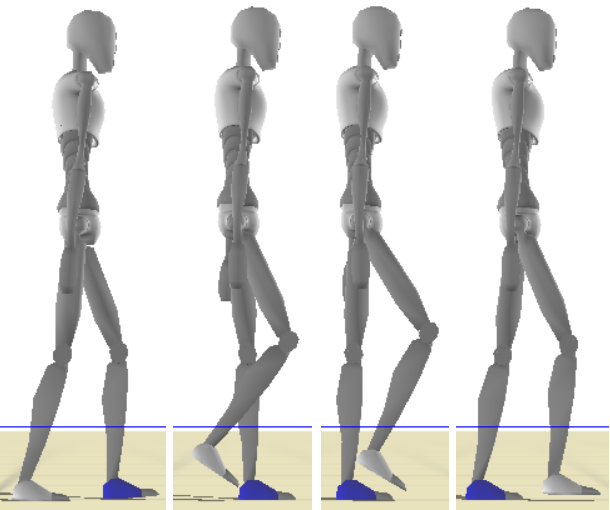
\includegraphics[scale=0.3]{strips/min_torque_25cm.png}
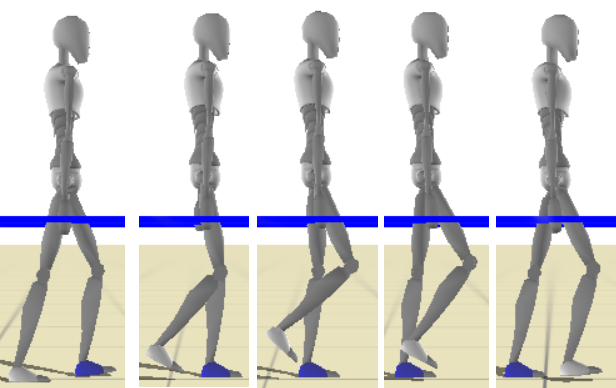
\includegraphics[scale=0.4]{strips/min_torque_75cm.png}
\caption{Marche d'un personnage cherchant à minimiser l'énergie dépensée dans 25cm d'eau (gauche) et dans 75cm d'eau (droite)}
\label{fig:min_energ}
\end{figure}


Ce critère ne prend en compte que l'énergie dépensée par le personnage. Les résultats que nous attendons sont des mouvements cherchant à produire le moins de rotations possible, n'essayant donc pas de sortir du liquide.

Comme nous nous y attendions le personnage lève très peu le pied en phase de vol lorsque le niveau de liquide est faible (figure \ref{fig:min_energ} (gauche)). Nous remarquons tout de même une augmentation de la hauteur des pas dès que le niveau du liquide atteint les genoux (figure \ref{fig:min_energ} (droite)). Ce changement est probablement due à l'action du liquide sur la jambe. Pour éviter de gaspiller de l'énergie en déplaçant le tibia avec un angle provoquant une forte opposition du liquide, le contrôleur préfère utiliser de l'énergie pour lever le pied de manière à aligner légèrement le tibias dans le sens du mouvement. 

\subsubsection{Étude de la minimisation de la résistance du liquide}

\begin{figure}[h]
\centering
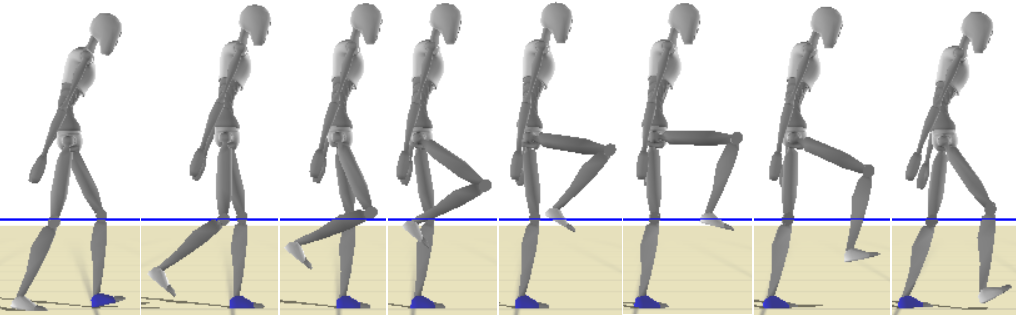
\includegraphics[scale=0.4]{strips/min_drag_75cm.png}
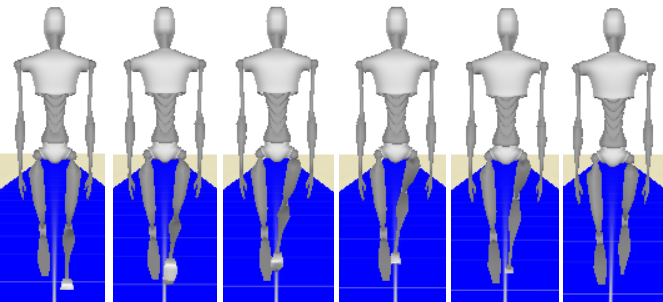
\includegraphics[scale=0.4]{strips/min_drag_25cm_from_back.png}
\caption{Marche d'un personnage cherchant à minimiser l'opposition de l'eau au mouvement dans 75cm d'eau (haut) et dans 25cm d'eau vue de dos (bas)}
\label{fig:min_drag2}
\end{figure}

Cette version ne prend en compte que la résistance de l'eau. Cela veux dire que pour une hauteur d'eau de 0m la fonction d'évaluation est inutile, ce qui fait que nous n'étudierons donc pas ce cas. Les résultats que nous attendons sont des mouvements cherchant à éviter un maximum le contact avec l'eau, donc un personnage cherchant à sortir les jambes de l'eau. On s'attend à apercevoir qu'après un certain niveau d'eau il devient impossible de sortir les jambes de l'eau et donc le personnage cherche à effectuer des mouvements les moins amples et les moins rapides possibles dans l'eau. 
 
Comme nous nous y attendions le personnage cherche bien à sortir le pied en phase de vol de l'eau (figure \ref{fig:min_drag_25}), ce phénomène est déjà presque impossible à une hauteur d'eau de 0,5m. Au dessus de 0,5m le contrôle choisit de ne plus lever la jambe et cherche à obtenir le mouvement optimal en restant au fond de l'eau (figure \ref{fig:min_drag_25} (gauche)). Il est également intéressant de noter que le personnage cherche à aligner le tibias dans le sens du déplacement pour éviter que l'eau n'applique une résistance dessus. Ce phénomène est particulièrement remarquable dans la phase de levée du pied. Pour les niveaux d'eau où le personnage cherche à sortir le pied hors de l'eau on remarque que le pied a une trajectoire assez courbée vers l'intérieur (figure \ref{fig:min_drag2} (droite)). Ce phénomène doit probablement servir à lever le pied aussi haut que possible mais il ne donne pas un résultat visuellement réaliste.  

\subsubsection{Minimisation des accélérations angulaires}
\begin{figure}[h]
\centering
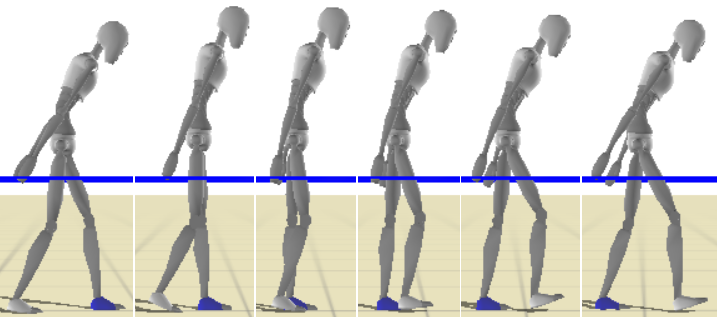
\includegraphics[scale=0.4]{strips/min_acc_75cm.png}
\caption{Marche d'un personnage cherchant à minimiser l'opposition les accélérations angulaires dans 75cm d'eau.}
\label{fig:min_acc}
\end{figure}

\begin{figure}[h]
\centering
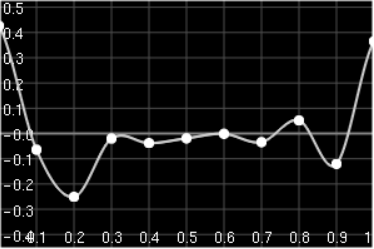
\includegraphics[scale=0.5]{strips/stance_ankle_min_torque.png}
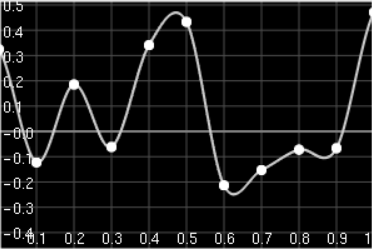
\includegraphics[scale=0.5]{strips/stance_ankle_min_acc.png}
\caption{Trajectoires cibles pour la cheville pour le critère de minimisation d'énergie (gauche) et le critère de minimisation des accélérations angulaires (droite)}
\label{fig:traj_ankle_min_torque}
\label{fig:traj_ankle_min_acc}
\end{figure}
Ce critère ne prend en compte que la composante pénalisant les accélérations élevées. Nous nous attendons à trouver un résultat proche de ceux obtenus pour le critère de minimisation de l'énergie. En effet, obtenir des accélérations élevées demanderait des torques élevés. La différence que nous attendons principalement est au niveau de la trajectoire désirée de la cheville d'appui. Nous nous attendons à observer une courbe bien plus lisse que celle observée pour le critère de minimisation de l'énergie.

On remarque que le mouvement obtenu lève le pied en phase de vol moins haut que lors de l'utilisation du critère de minimisation de l'énergie. On remarque également que cette fonction pousse plus à pencher le torse pour gagner de la vitesse.
 Contrairement à ce que nous espérions nous observons toujours des variations importantes sur la trajectoire de la cheville d'appui avec ce critère (voir figure \ref{fig:traj_ankle_min_acc} (droite)). C'est peut être du au fait que le personnage garde le pied extrêmement proche du sol au cours du mouvement. La courbe à donc probablement appris les variations permettant de rester aussi proche que possible du sol sans le toucher.


Nous allons maintenant étudier quelques combinaisons de la fonction d'évaluation (équation \ref{eq:complete_eval}). Nous utiliserons la dénomination suivante lorsque nous voulons nous référer à une des combinaisons $f(\alpha,\beta,\gamma)$. Dans cette partie nous ne réétudierons pas les niveaux d'eau pour lesquels les résultats étaient similaires pour les trois critères d'optimisation (0, 0.75 et 1) car toute combinaison des résultats donnerait le même résultat. Donc nous n'étudierons que les niveaux de liquide 0,25m et 0,5m. Le but de cette étude est de trouver une combinaison permettant d'obtenir un mouvement fortement conditionné par la présence du liquide, dépensant une quantité d'énergie assez faible et ne présentant pas d'accélérations brusques. 

\subsubsection{Étude de f(2,8,1)}

\begin{figure}[h]
\centering
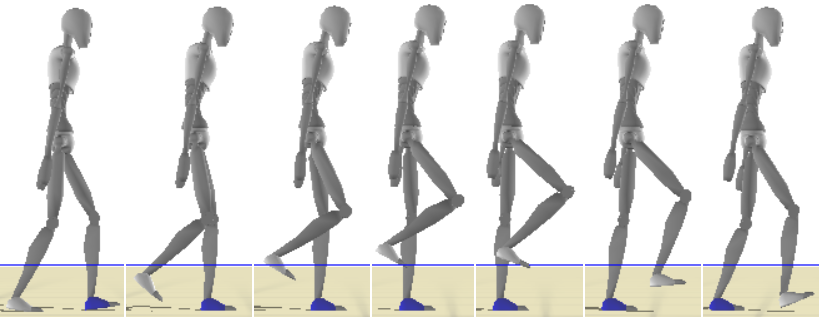
\includegraphics[scale=0.35]{strips/2_8_1_25cm.png}
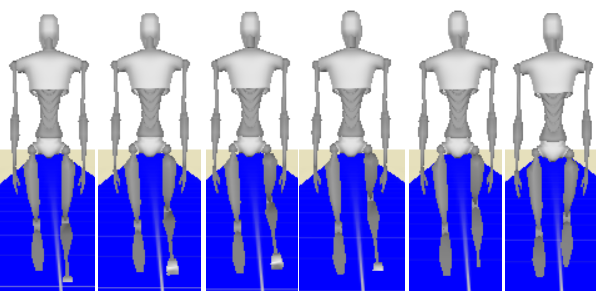
\includegraphics[scale=0.35]{strips/2_8_1_25cm_from_back.png}
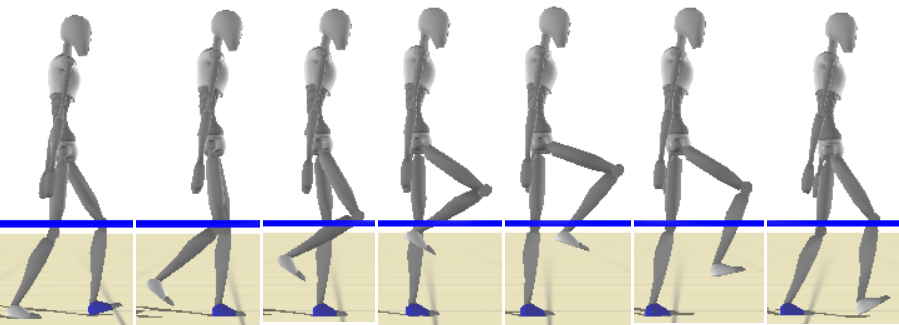
\includegraphics[scale=0.4]{strips/2_8_1_50cm.png}
\caption{Marche d'un personnage selon la fonction d'évaluation f(2,8,1) dans 25cm de liquide vu de coté (gauche) et vu de dos (droite) et dans 50cm de liquide vu de coté (bas). }
\label{fig:f281}
\end{figure}

Tout d'abord on remarque que l'on conserve bien les caractéristiques du critère de minimisation de la résistance du liquide, c'est à dire que le personnage lève le pied même pour une hauteur de liquide élevée (figure \ref{fig:f281} (gauche) et figure \ref{fig:f281} (bas)). Cependant on remarque qu'il y a toujours le mouvement latéral du pied en phase de vol sur une hauteur de 0.25m de liquide (voir figure \ref{fig:f281} (droite)). Nous allons donc tenter de diminuer l'influence du critère de minimisation de la résistance du liquide pour faire disparaître ce mouvement latéral.

\subsubsection{Étude de f(3,6,1)}
\begin{figure}[h]
\centering
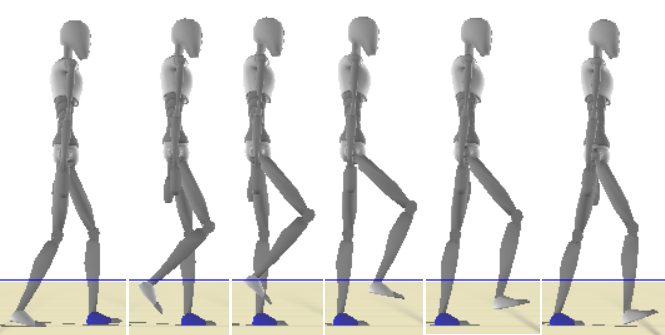
\includegraphics[scale=0.35]{strips/3_6_1_25cm.png}
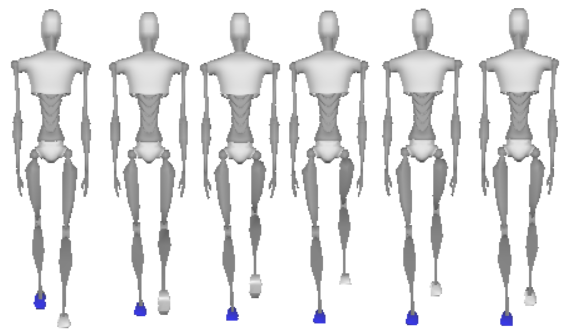
\includegraphics[scale=0.35]{strips/3_6_1_25cm_from_back.png}
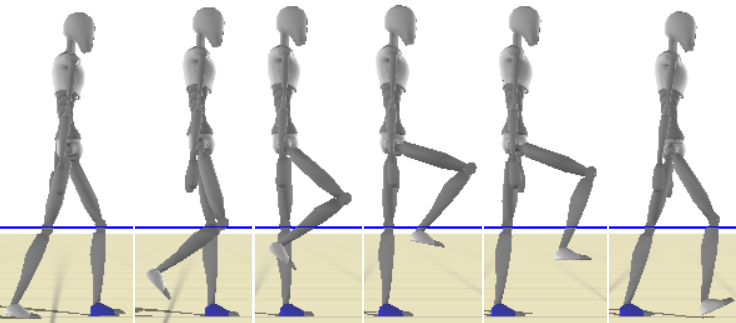
\includegraphics[scale=0.4]{strips/3_6_1_50cm.png}
\caption{Marche d'un personnage selon la fonction d'évaluation f(3,6,1) dans 25cm de liquide vu de coté (gauche) et vu de dos (droite) et dans 50cm de liquide vu de coté (bas)}
\label{fig:f361}
\end{figure}

Nous constatons que cette fois-ci il n'y a pas de mouvement latéral sur le pied lors de la marche dans 0.25m de liquide (voir figure \ref{fig:f361} (droite)). Nous avons toujours un mouvement fortement conditionné par l'impact du liquide (figure \ref{fig:f361} (gauche) et (bas)). Cependant on remarque tout de même que le personnage ne sort plus le pied du liquide lors de l'immersion dans 0.25m de liquide (figure \ref{fig:f361} (gauche)). Nous allons maintenant voir si diminuer encore l'influence du critère de minimisation de la résistance du liquide à une influence sur le résultat ou si celui-ci reste stable.

\subsubsection{Étude de f(4,5,1)}
\begin{figure}[h]
\centering
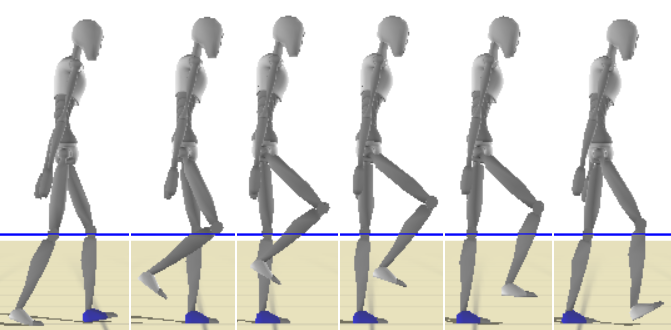
\includegraphics[scale=0.4]{strips/4_5_1_50cm.png}
\caption{Marche d'un personnage selon la fonction d'évaluation f(4,5,1) dans 50cm de liquide.}
\label{fig:f451}
\end{figure}

On remarque que cette combinaison de paramètre diminue la hauteur à laquelle le pied est levé même si celui-ci ne sort pas du liquide avec la fonction f(3,6,1) (voir figure \ref{fig:f451}). Nous sommes donc moins intéressé ces valeurs de poids. 

\subsection{Étude du contrôleur complexe}

Au vu des résultats précédents nous utilisons la fonction d'évaluation f(3,6,1) pour la création du contrôleur complexe. Ce contrôleur sera créés en utilisant les trajectoires spécifiques aux vitesses $0,3m*s^{-1}$ et $0,7m*s^{-1}$. Nous utilisons un système similaire à celui utilisé pour la combinaison des courbes de vitesse pour combiner les courbes spécifiques à un niveau de liquide. Donc pour chacune des vitesses de référence nous aurons 5 trajectoires, une pour chacun des niveaux de liquide suivants 0cm, 25cm, 50cm, 75cm, 100cm. Ce contrôleur permet une animation en temps réel. Nous observons un minimum de 27fps sur la totalité de nos conditions d'expérimentation.

Avant de créer notre contrôleur nous allons vérifier si l'on ne peut pas trouver une relation entre les trajectoires des différents niveaux de liquide utilisées par une articulation. L'existence de telles relations nous permettrait de créer un contrôleur générique pour toute hauteurs d'eau. Dans un premier temps nous allons regarder d'une manière globale si on peut trouver des articulations avec des trajectoires similaires sur plusieurs niveaux de liquide. Dans un second temps nous regarderons pour chaque point des trajectoires si l'on ne peut pas trouver une relation linéaire décrivant son évolution entre les différents niveaux de liquide.

\begin{figure}[h]
\centering
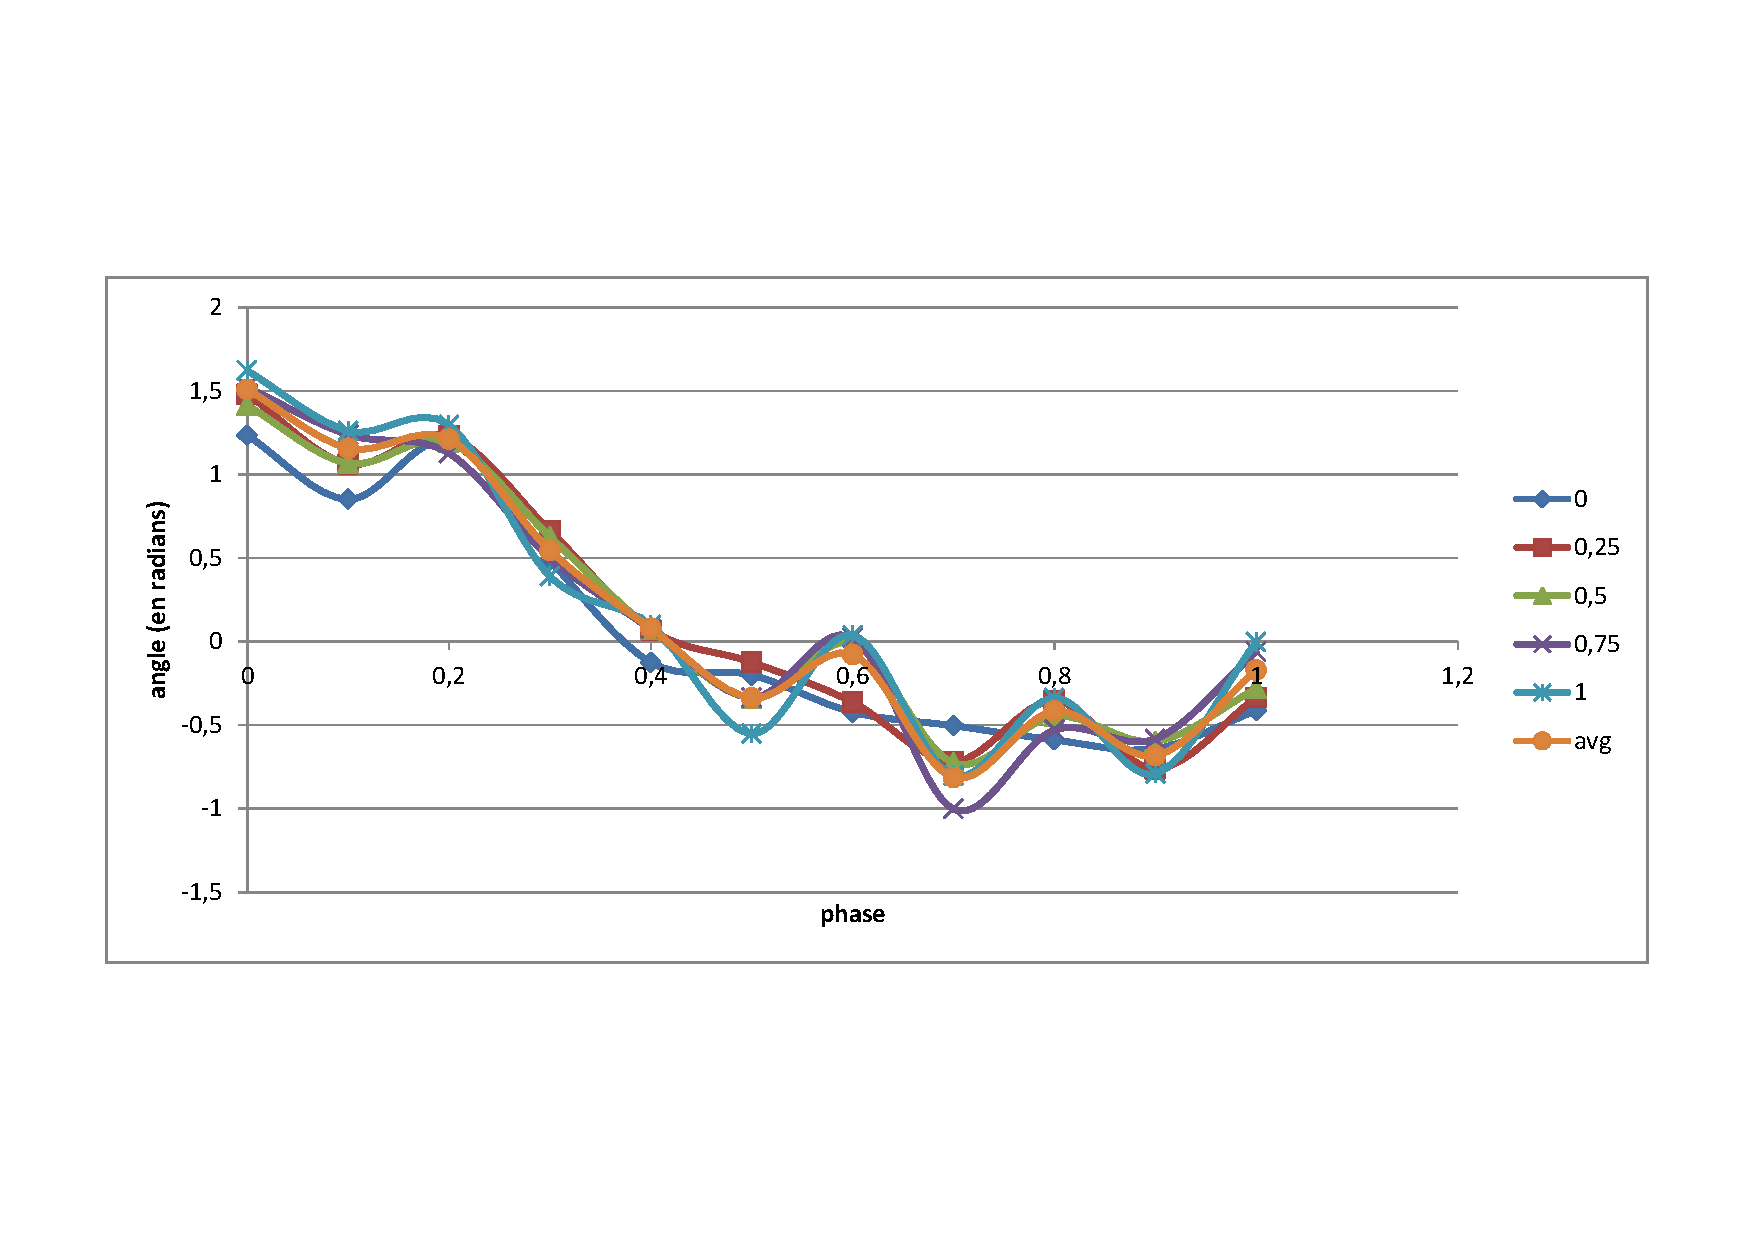
\includegraphics[scale=0.4]{trajs_swing_ankle.pdf}
\caption{Comparaison des trajectoires cibles pour chaque niveau de liquide (en mètres) de la cheville en phase de vol. La trajectoire $avg$ est une moyenne des autres trajectoires à l'exception de la trajectoire du niveau de liquide 0m car trop différente des autres.}
\label{fig:comp_traj_swing_foot}
\end{figure}

Nous ne trouvons une similarité entre les trajectoire de références pour divers niveaux de liquide que pour l'articulation de la cheville en phase de vol (figure \ref{fig:comp_traj_swing_foot}). On peut voir sur le graphique qu'à l'exception de la courbe correspondant au personnage sans liquide les courbes sont très similaires. Nous avons donc calculé la moyenne des courbes en ne prenant pas en compte le niveau de liquide 0m et utilisons cette nouvelle courbe en temps que trajectoire pour toutes les courbes de références des niveaux de liquides supérieurs ou égal à 0.25m. 

\begin{figure}[h]
\centering
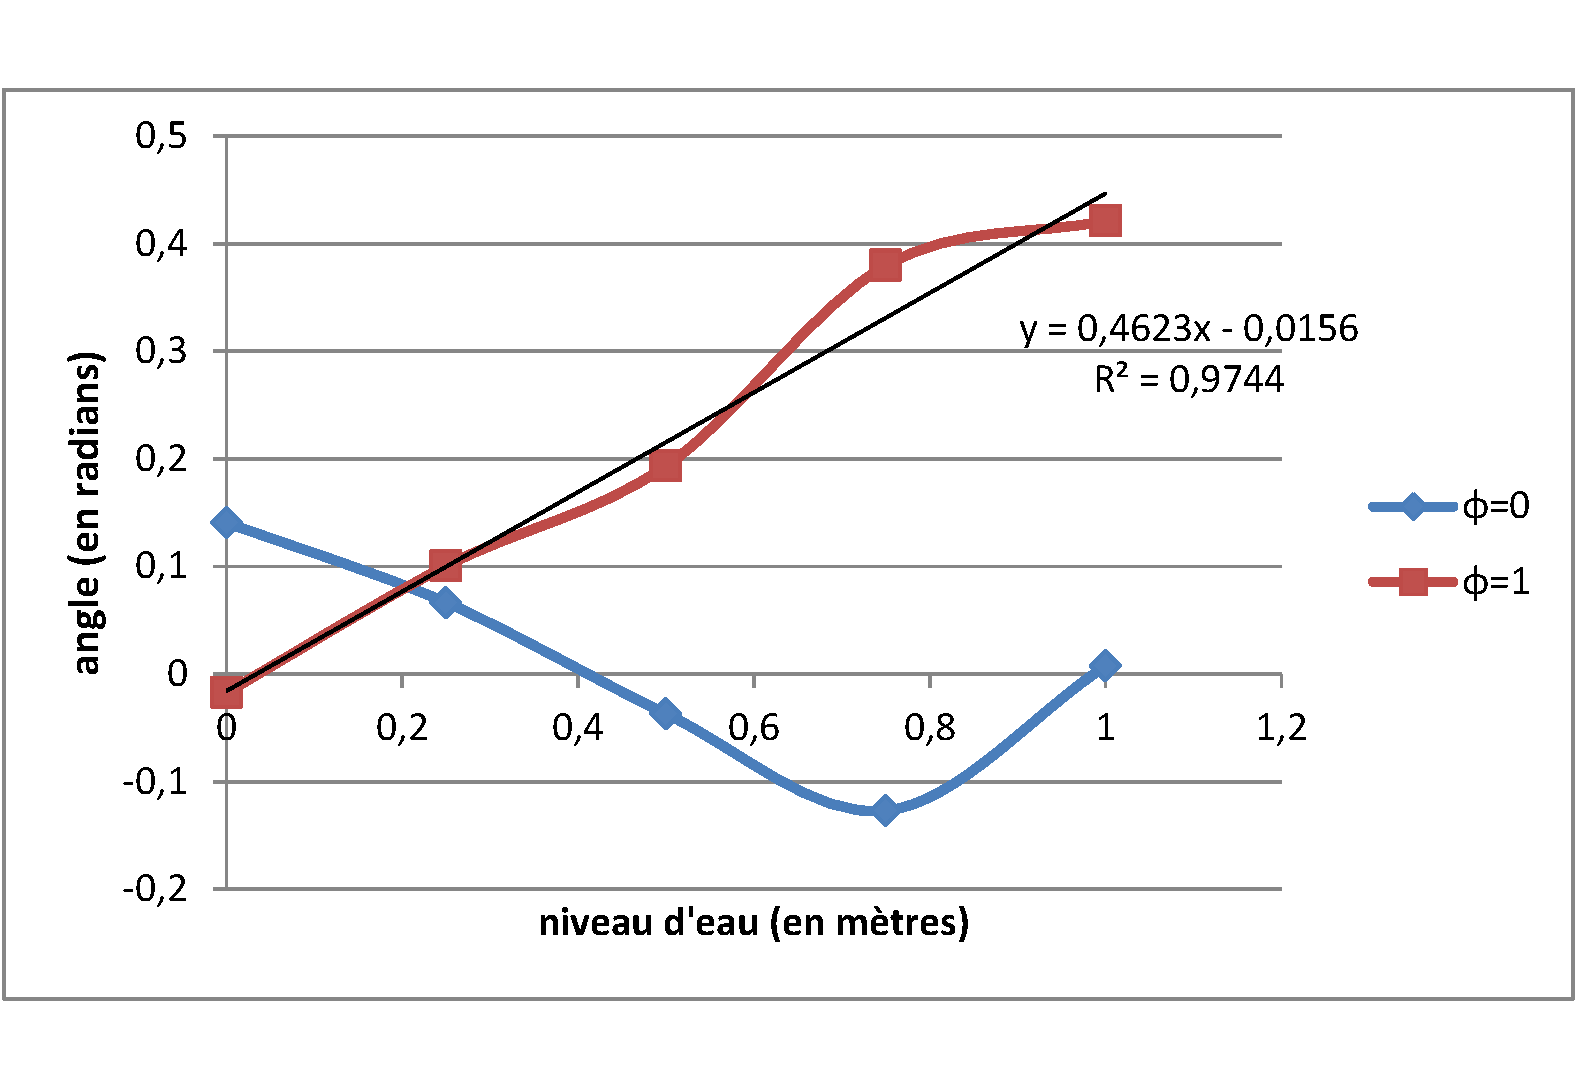
\includegraphics[scale=0.27]{img_curve_pelvis_torso.pdf}
\caption{Variations des points clefs de la trajectoire de l'articulation entre le pelvis et le torse. On remarque une corrélation linéaire pour le point correspondant à $\phi=1$}
\label{fig:img_curve_pelvis_torso}
\end{figure}

Nous avons ensuite effectué une étude de l'évolution de l'angle de chaque point en fonction de la hauteur de liquide (voir annexe \ref{sec:evo_key_points_with_wlvl}). Nous ne considérons pas la cheville en phase de vol car nous avons déjà proposé une solution pour prendre en compte les similitudes. On remarque que les points présentant une relation entre les niveaux de liquide sont isolés les uns des autres. Nous pouvons tout de même observer que le point clef final de la trajectoire de l'articulation entre le pelvis et le torse est fortement corrélé avec la hauteur de liquide (voir figure \ref{fig:img_curve_pelvis_torso}). Cette trajectoire n'étant composé que de deux points clefs il nous semble intéressant de prendre en compte cette corrélation. Cette observation est particulièrement intéressante car cette trajectoire à un grand impact sur le mouvement du fait de la masse importante du torse. Nous implémentons cette corrélation à travers un système qui modifiera ce point dans les trajectoires selon la formule suivante $\theta_d=0.4623h-0.0156$ avec $h$ la hauteur de liquide.

\subsubsection{Contrôle du personnage et interactions avec l'environnement}

Notre contrôleur permet la variation dynamique des vitesses désirées suivant les axes sagittal et coronal. Il est également possible de modifier la largeur des pas au cours du mouvement.
Le contrôleur est capable de s'adapter aux variations de niveau de liquide ainsi qu'aux variations de propriétés physiques du liquide (densité, viscosité). Notre système est capable de supporter des forces externes simulées par l'intermédiaire de boules solides de 5kg projetées sur le personnage.

Tous ces résultats sont présentés dans la vidéo accompagnant ce document (trouvable à l'adresse précédemment mentionnée). 


\subsection{Limitations}
Notre contrôleur possède plusieurs limitations provenant de diverses origines. Une limitation majeure de notre système est la présence d'un seuil fixe permettant la détection des instabilités. Il est très dur d'obtenir un seuil adapté car suivant la situation il serait préférable d'avoir un seuil plus ou moins élevé. Durant la phase de convergence vers le mouvement stable il nous est nécessaire d'avoir un seuil élevé pour permettre au système d'évoluer assez rapidement à partir d'une position initiale potentiellement non adaptée au mouvement. Mais l'utilisation d'un seuil élevé lors de la phase d'équilibre empêche  une réaction efficace du personnage. 
Une seconde limitation de notre système est qu'il n'assure pas un contact ferme entre le pied d'appui et le sol. Ce phénomène est du au fait qu'il est très difficile d'obtenir une trajectoire de la cheville d'appui assurant un maintien correct du contact avec le sol. Il est fréquent que lors de nos simulations le personnage arrive à faire glisser le pied au sol. Ce phénomène est particulièrement visible lorsque l'on introduit un déséquilibre à l'aide d'une force externe. 
Une troisième limitation est le besoin de définir plusieurs ensembles de trajectoires pour permettre un suivi correct de la vitesse en gardant un mouvement naturel. 
Enfin le modèle simplifié que nous avons utilisé pour la simulation du liquide ne nous permet pas d'assurer que les mouvement obtenus sont parfaitement réalistes. Nous ne prenons pas en compte les perturbations du liquide provoquées par le personnage alors qu'il est probable que celle-ci soient non négligeables. Cette remarque est particulièrement justifiée pour les mouvement ou le personnage élève le pied en phase de vol hors du liquide ce qui provoque probablement des perturbations importantes du liquide.
 %L'ajout de contrôleurs supplémentaires sur les articulations clefs telles que la cheville d'appui permettrait %de gagner en robustesse du mouvement. Une amélioration de la capacité à détecter la perte d'équilibre %permettrait également au système de gagner grandement en robustesse.
\section{Conclusion}
\label{sec:conclusion}
%
Nous avons présenté un contrôleur basé physique permettant l'animation d'un personnage bipède à travers un milieu liquide. Notre contrôleur se sert d'un ensemble de trajectoires cibles pour pouvoir adapter son style de déplacement aux conditions de l'environnement. Nous obtenons une marche robuste et un suivi précis de la vitesse désirée par l'intermédiaire d'un placement intelligent du pied et de l'utilisation de systèmes incrémentaux pour prendre en compte l'influence de l'environnement. Enfin nous avons utilisé une méthode d'optimisation hors ligne pour obtenir un déplacement caractéristique des différents niveaux de liquide considérés.
Nous avons proposé une paramétrisation de notre contrôleur permettant l'adaptation dynamique du mouvement aux variations de vitesse désirée, aux changements de quantité de liquide ainsi qu'à la modification des propriétés physiques de ce dernier. Nous avons également montré un maintien de l'équilibre après application de forces externes.

Nous pensons que des extensions du contrôleur sont possibles. Il serait intéressant de mettre en place un modèle plus réaliste pour les liquides ainsi que des milieux déformables (tel que la neige) pour déterminer quels sont les composants manquants au système pour obtenir un déplacement réaliste. Enfin l'extension de notre contrôleur à de nouveaux déplacements tel que la course ou des mouvement en position statique est une piste de travail intéressante. 

Un article présentant les résultats de ce stage est en cours de rédaction pour être soumis à la conférence internationale Motion In Games 2015.
%



%
\nocite{*}
\bibliographystyle{splncs03}
\bibliography{references}
%
\newpage

\appendix
\section{Lexique}
\label{sec:lexique}
\subsubsection{pas.} Nous définissons un pas comme le mouvement permettant de déplacer un pied en contact avec le sol à une nouvelle position présentant un contact avec le sol

\subsubsection{phase de vol.} Un élément est dit en phase de vol quand il fait partit de la jambe n'ayant pas de contact avec le sol.

\subsubsection{phase d'appui.} Un élément est dit en phase d'appui quand il fait partit de la jambe ayant un contact avec le sol.

\subsubsection{phase du pas ($\phi$).} Nous définissons la phase du pas comme le rapport entre le temps $t$ écoulé depuis le début du pas et le temps maximum $T$ autorisé pour réaliser un pas $\phi=\frac{t}{T}$


\section{Visualisation des styles de marches du contrôleur pour les hauteurs de liquide et les vitesses de références}
\label{sec:complex_controler}

\newpage
\section{Courbes d'évolution des points clefs des trajectoires de référence en fonction du niveau de liquide}
\label{sec:evo_key_points_with_wlvl}
\begin{figure}[h]
\centering
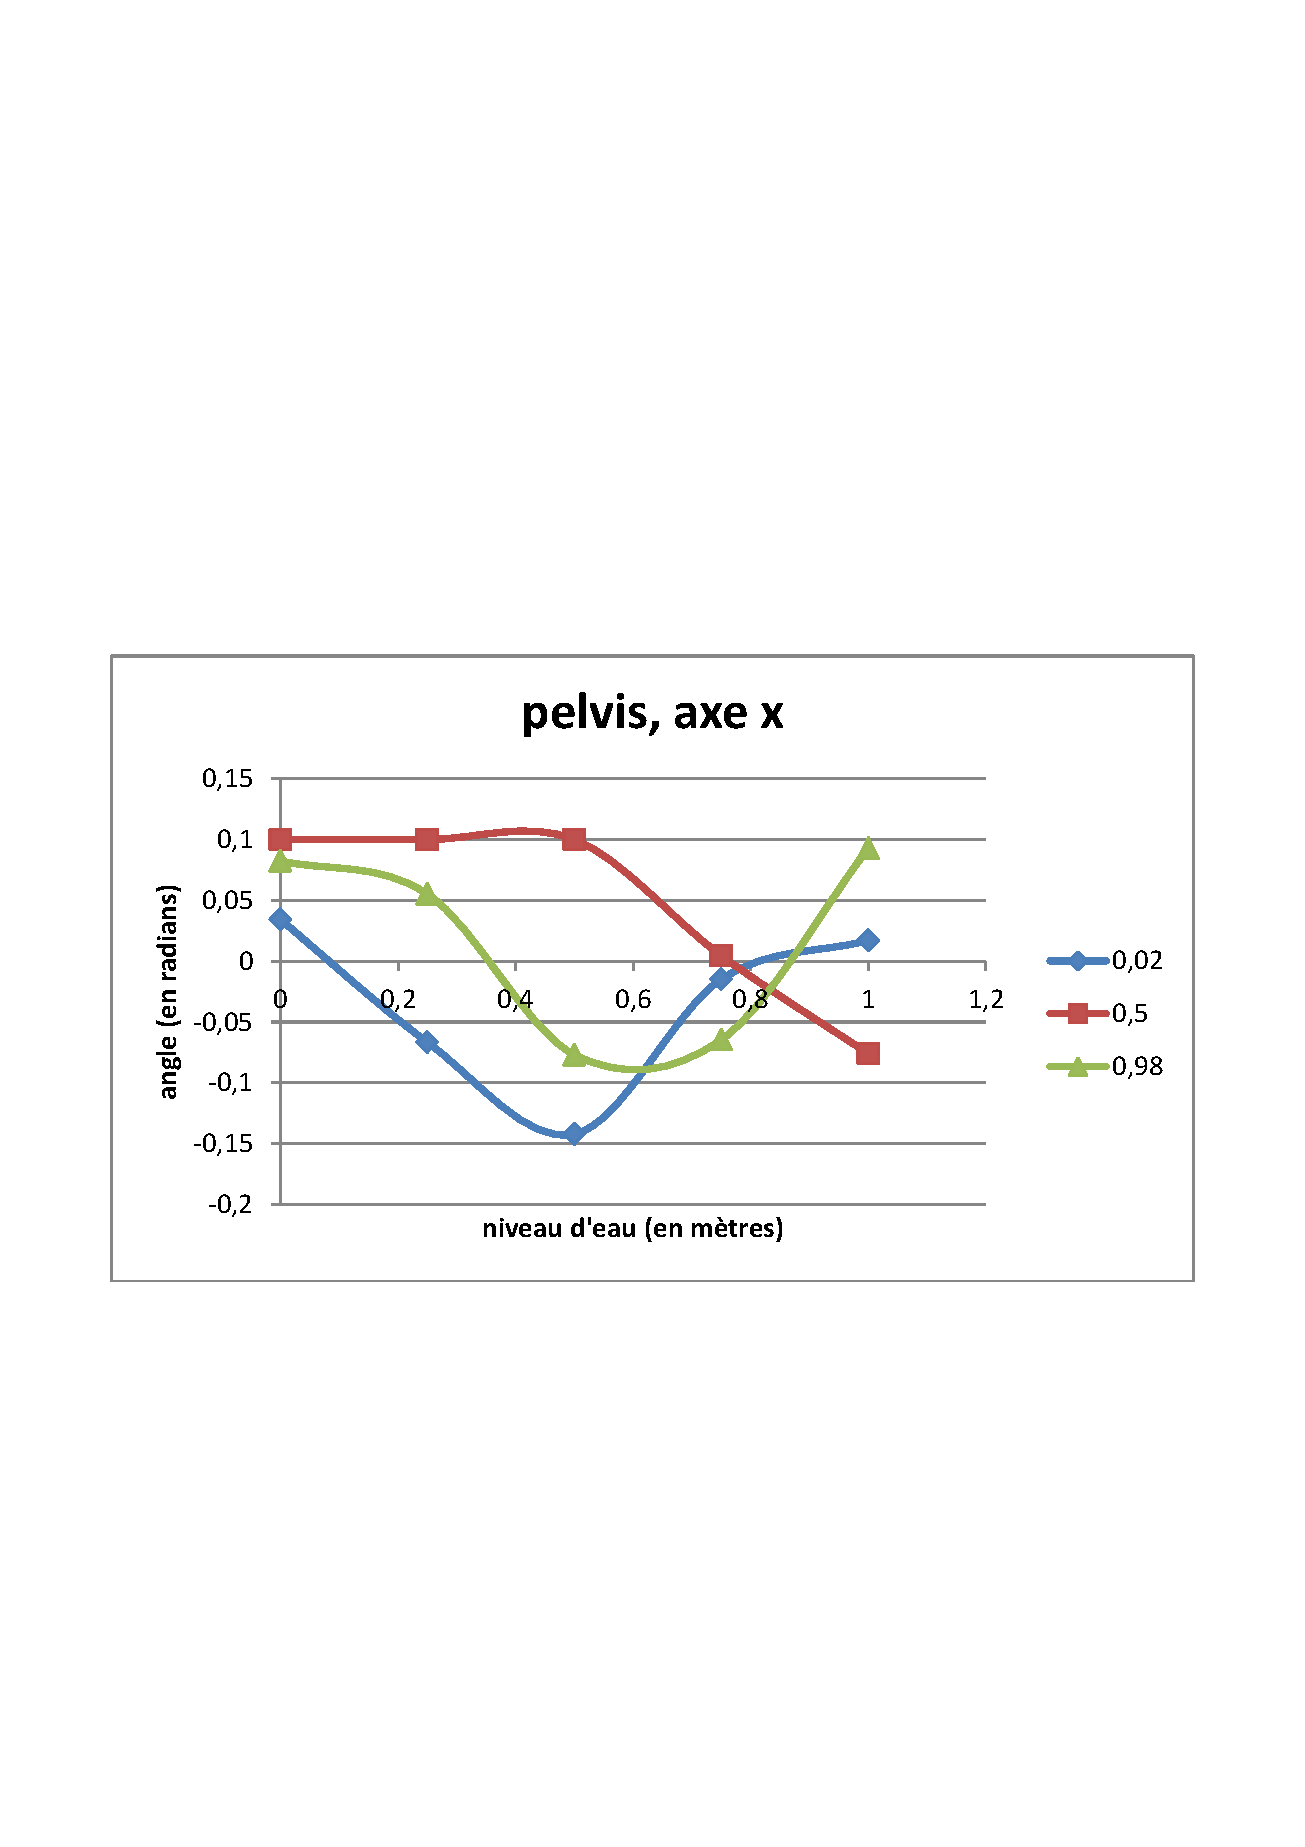
\includegraphics[scale=0.3]{traj_pts_clefs/pelvis_x.pdf}
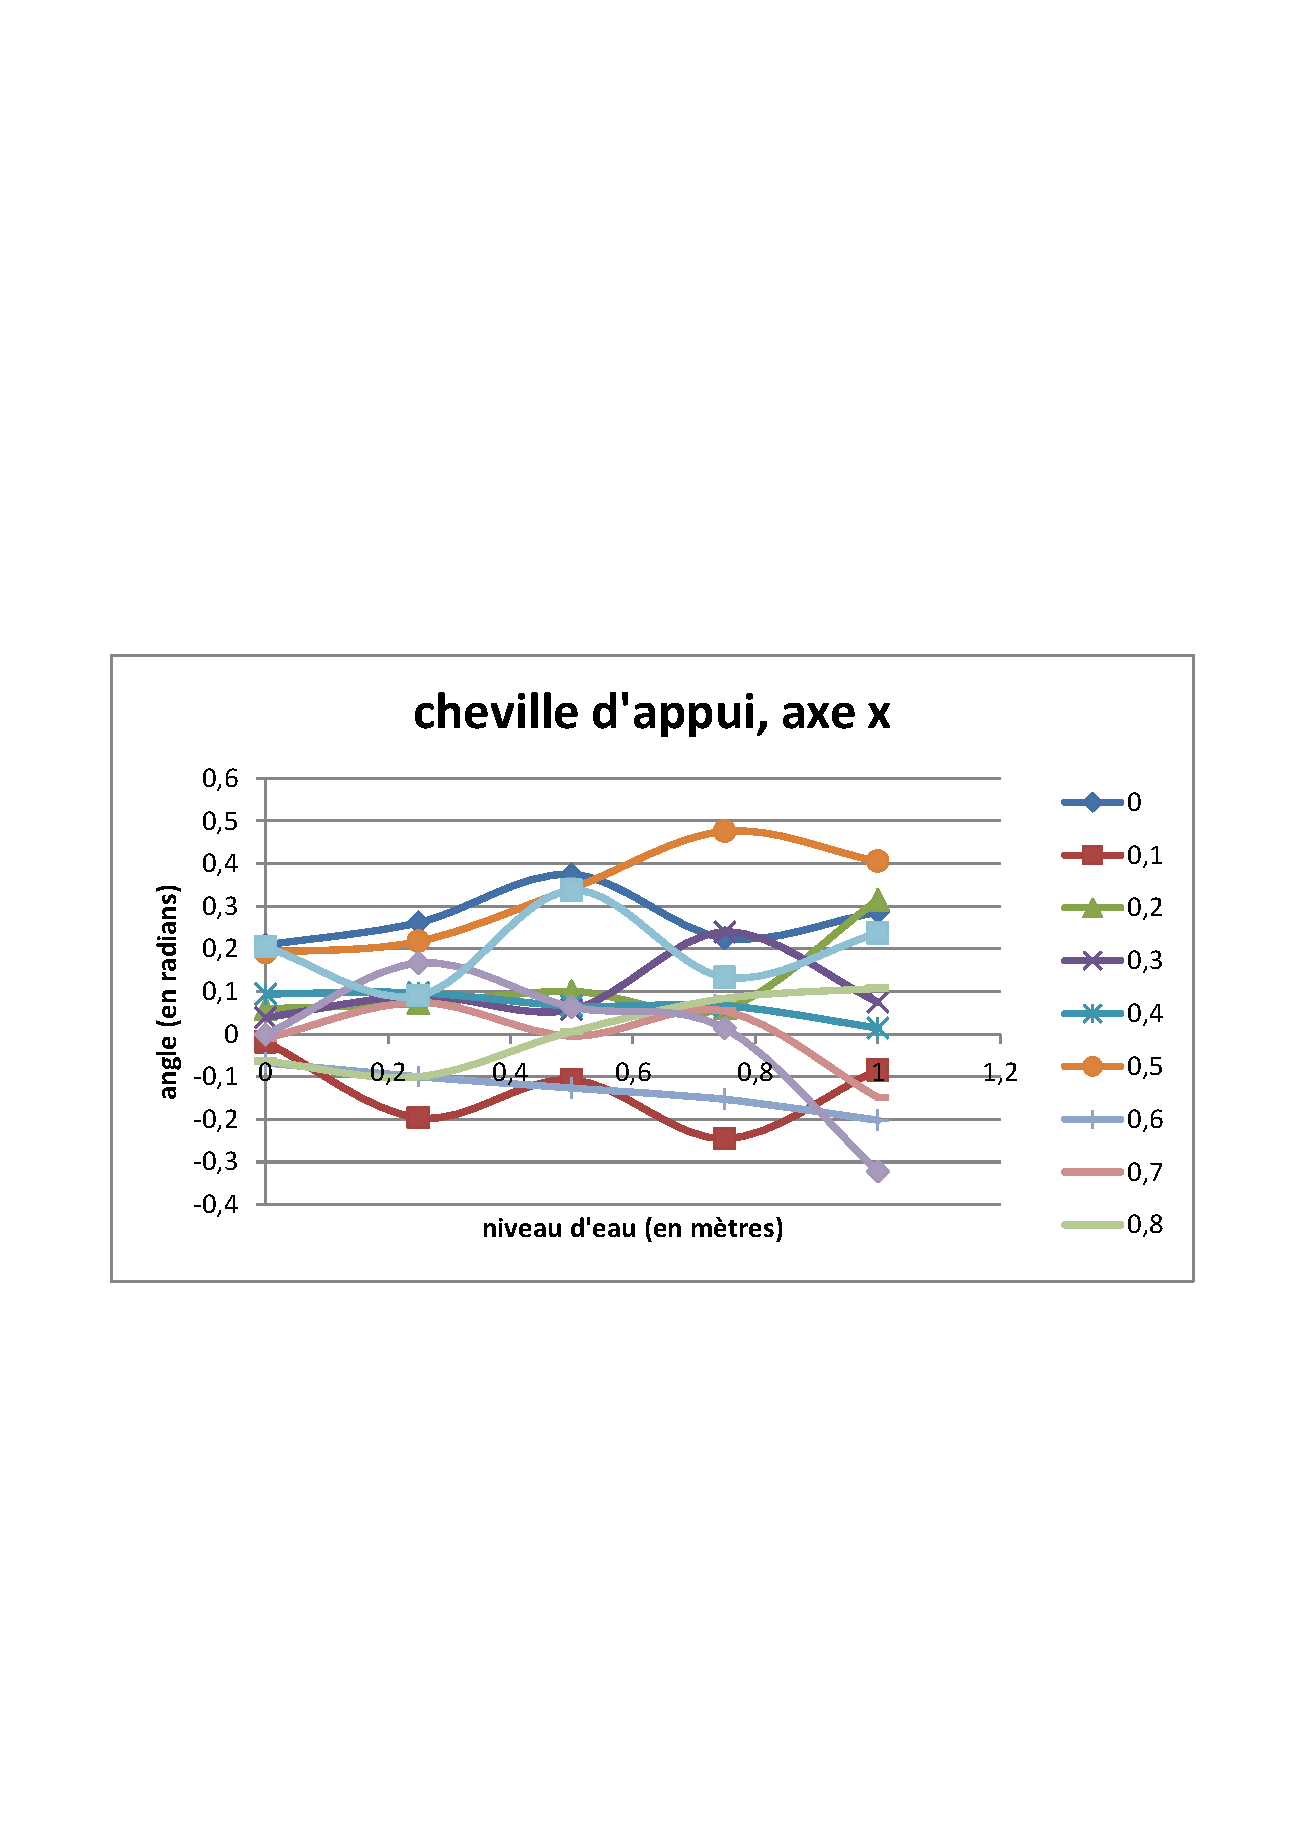
\includegraphics[scale=0.3]{traj_pts_clefs/stance_ankle_x.pdf}
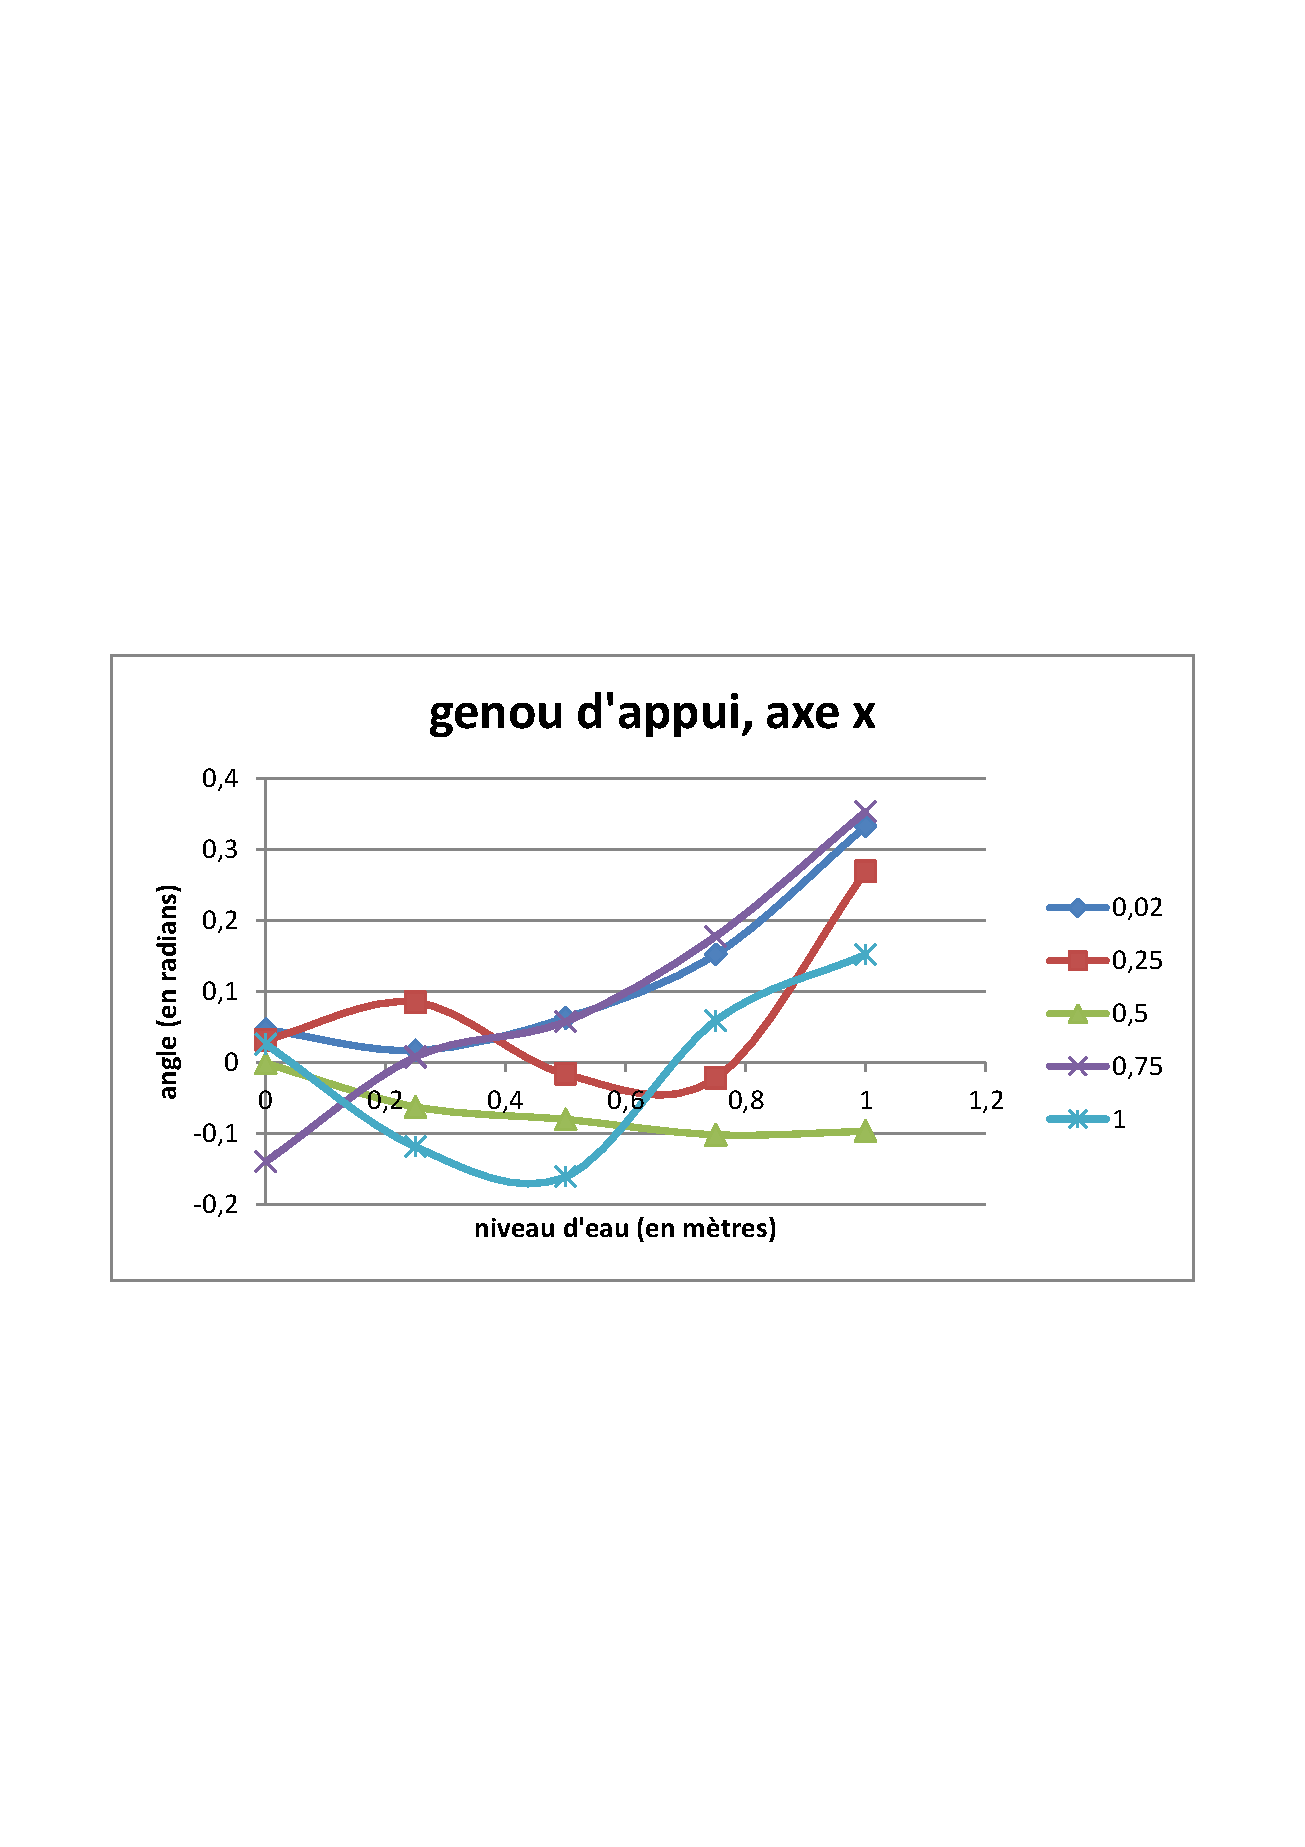
\includegraphics[scale=0.3]{traj_pts_clefs/stance_knee_x.pdf}
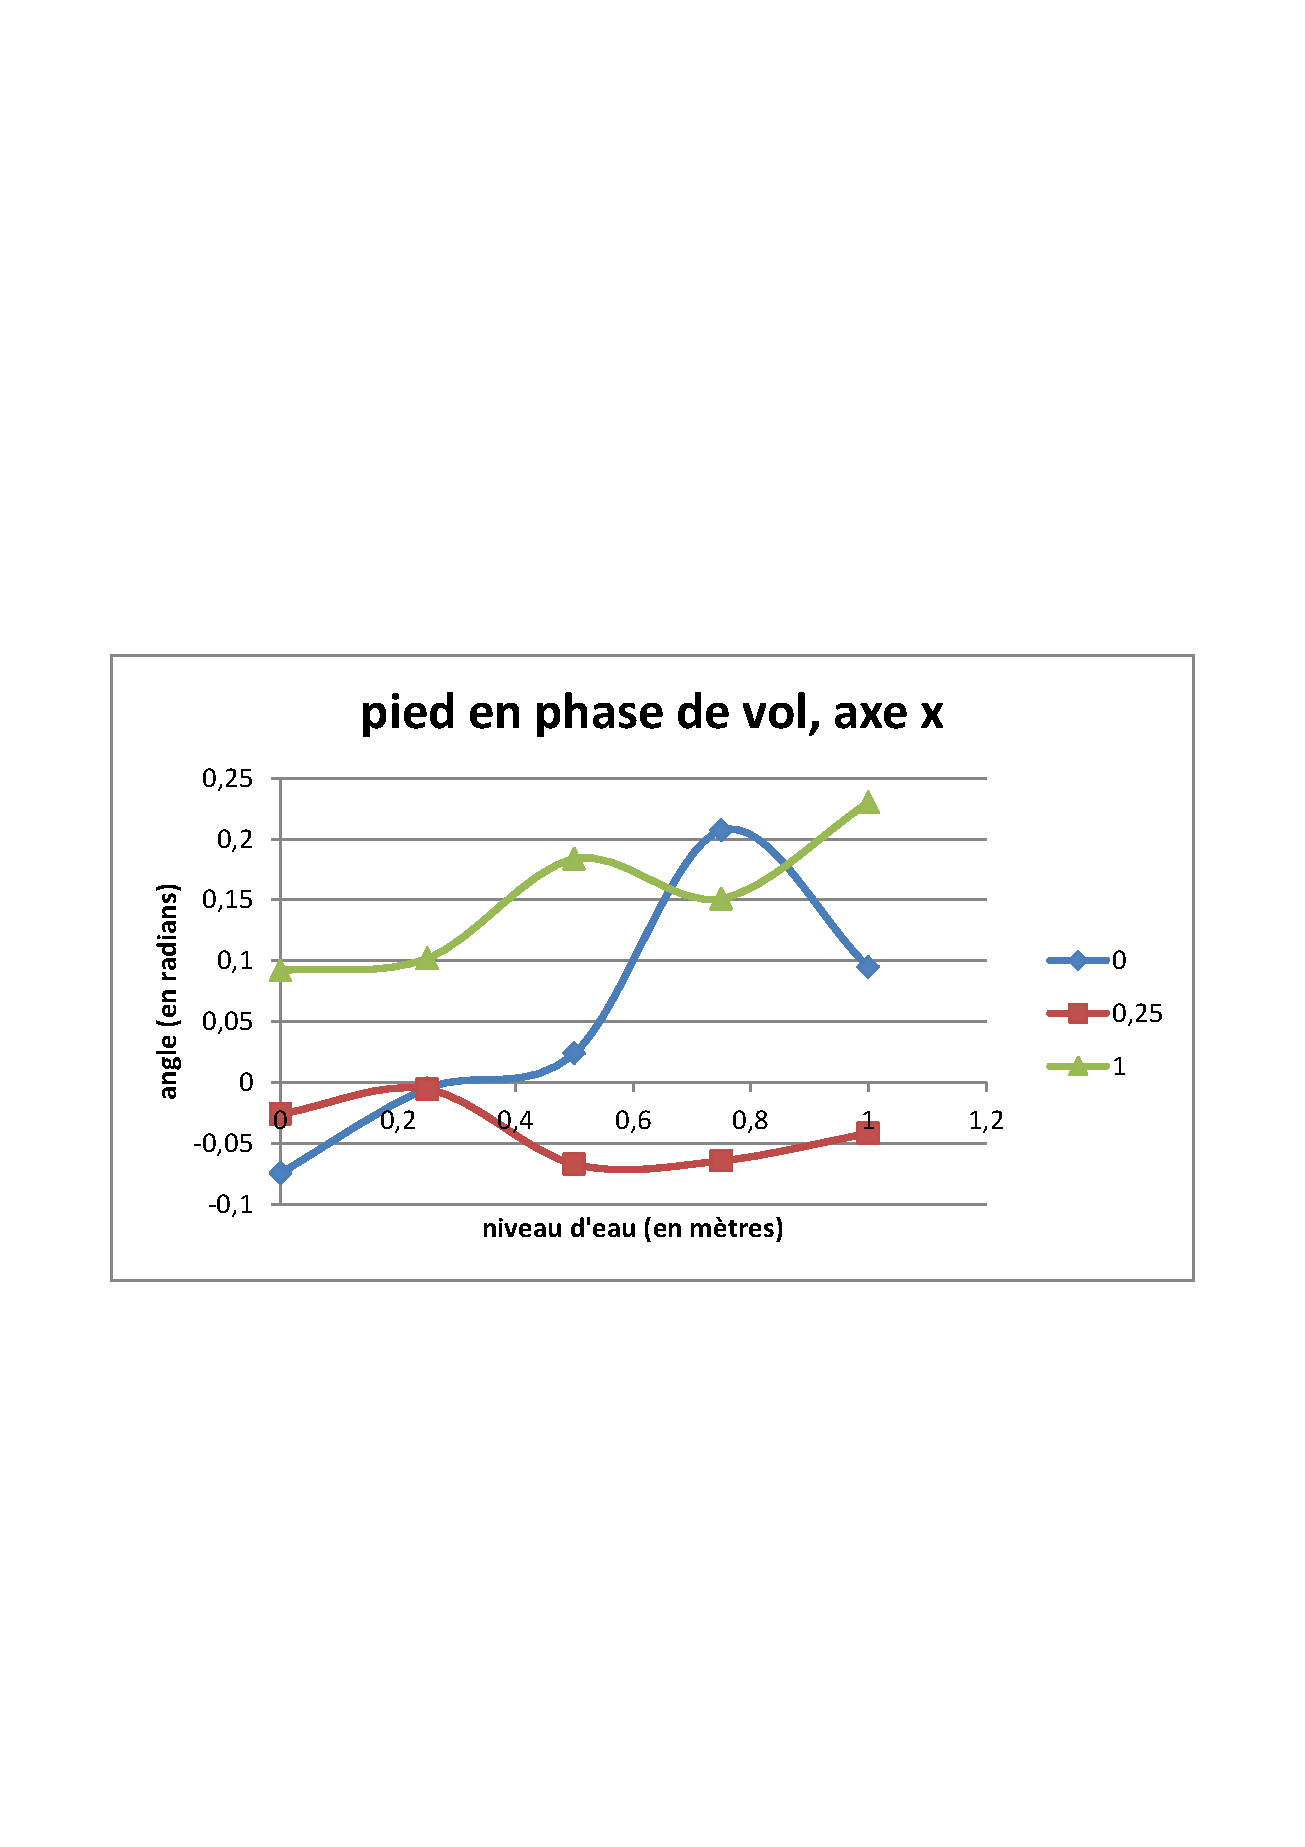
\includegraphics[scale=0.3]{traj_pts_clefs/swing_foot_x.pdf}
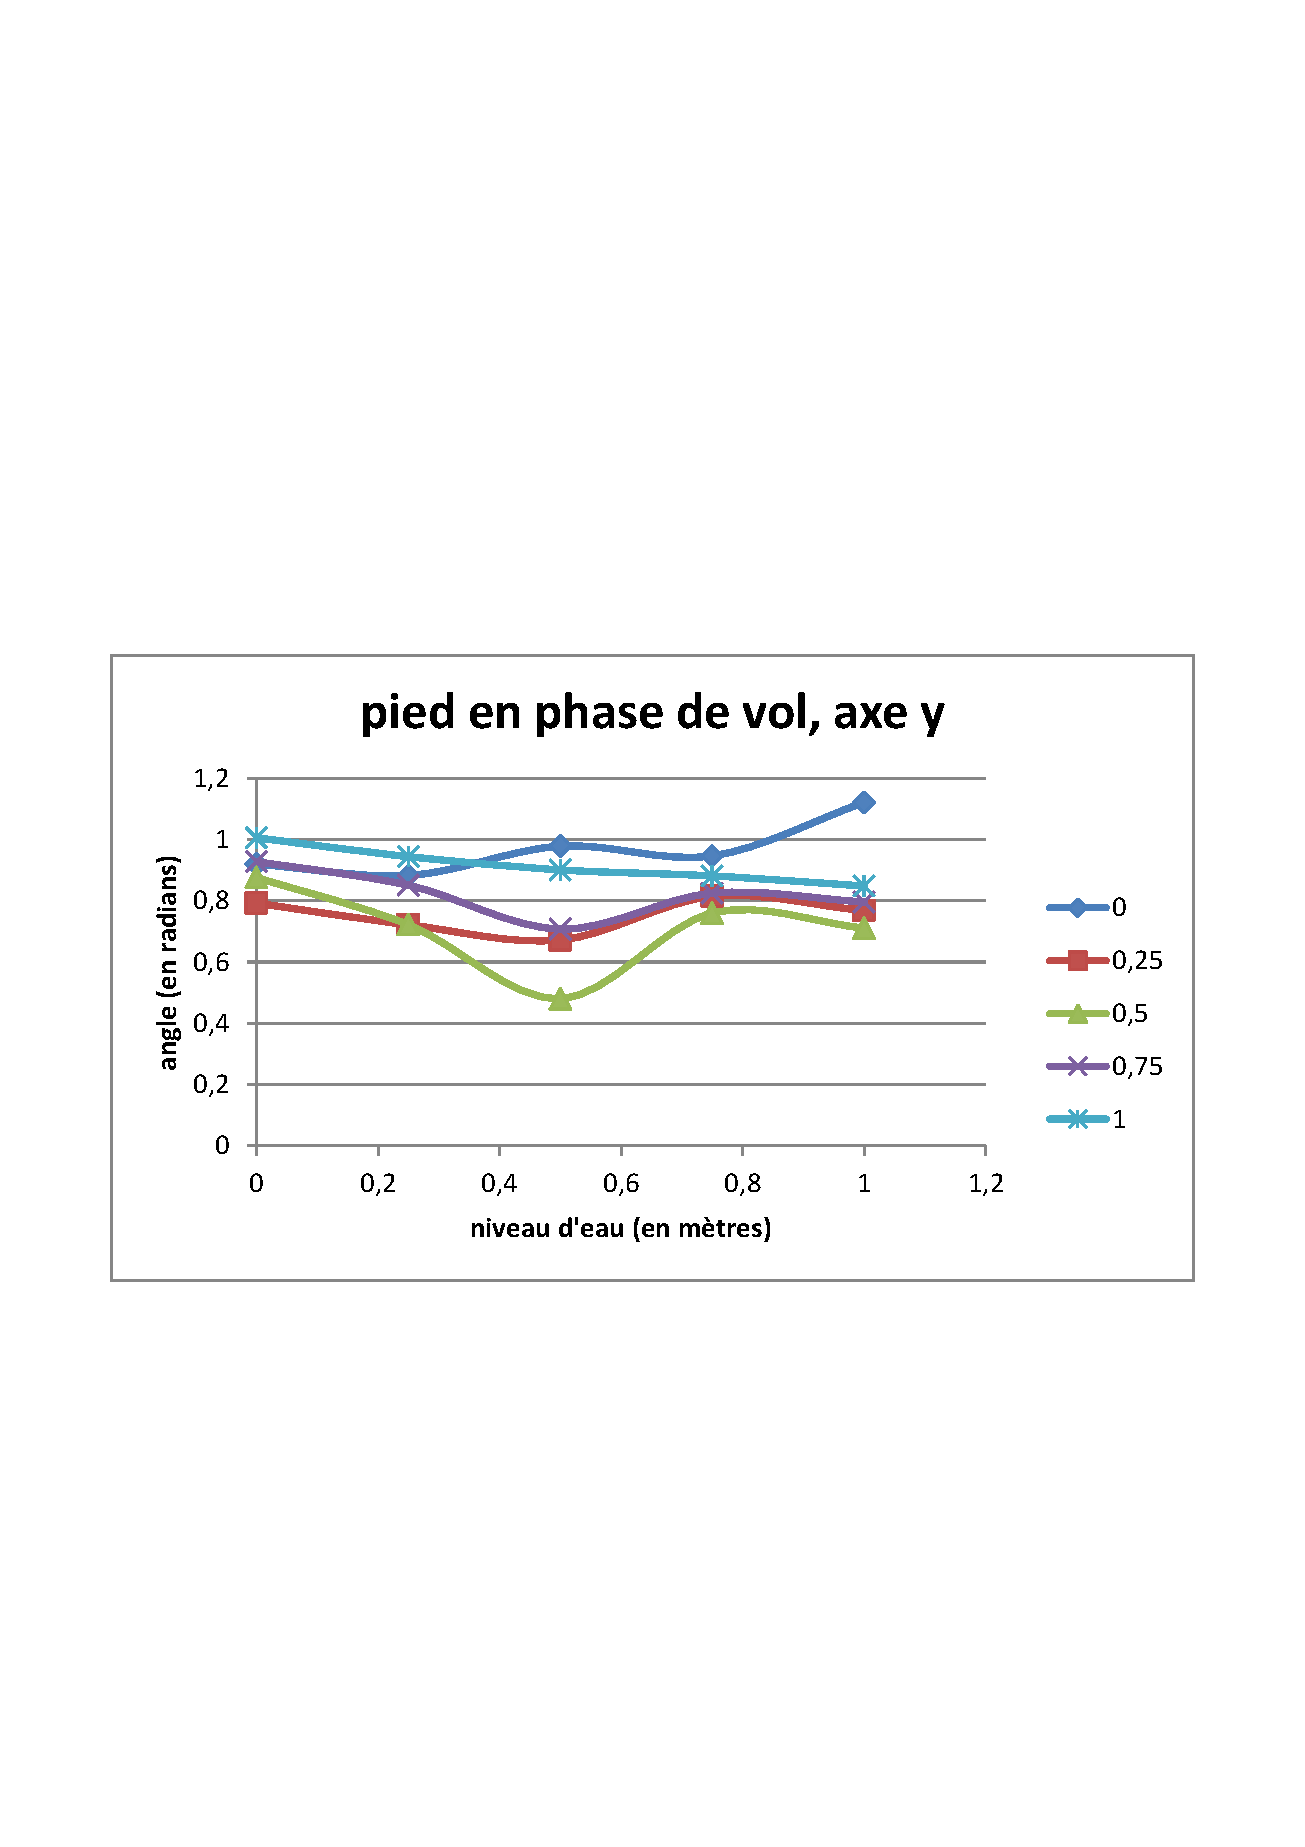
\includegraphics[scale=0.3]{traj_pts_clefs/swing_foot_y.pdf}
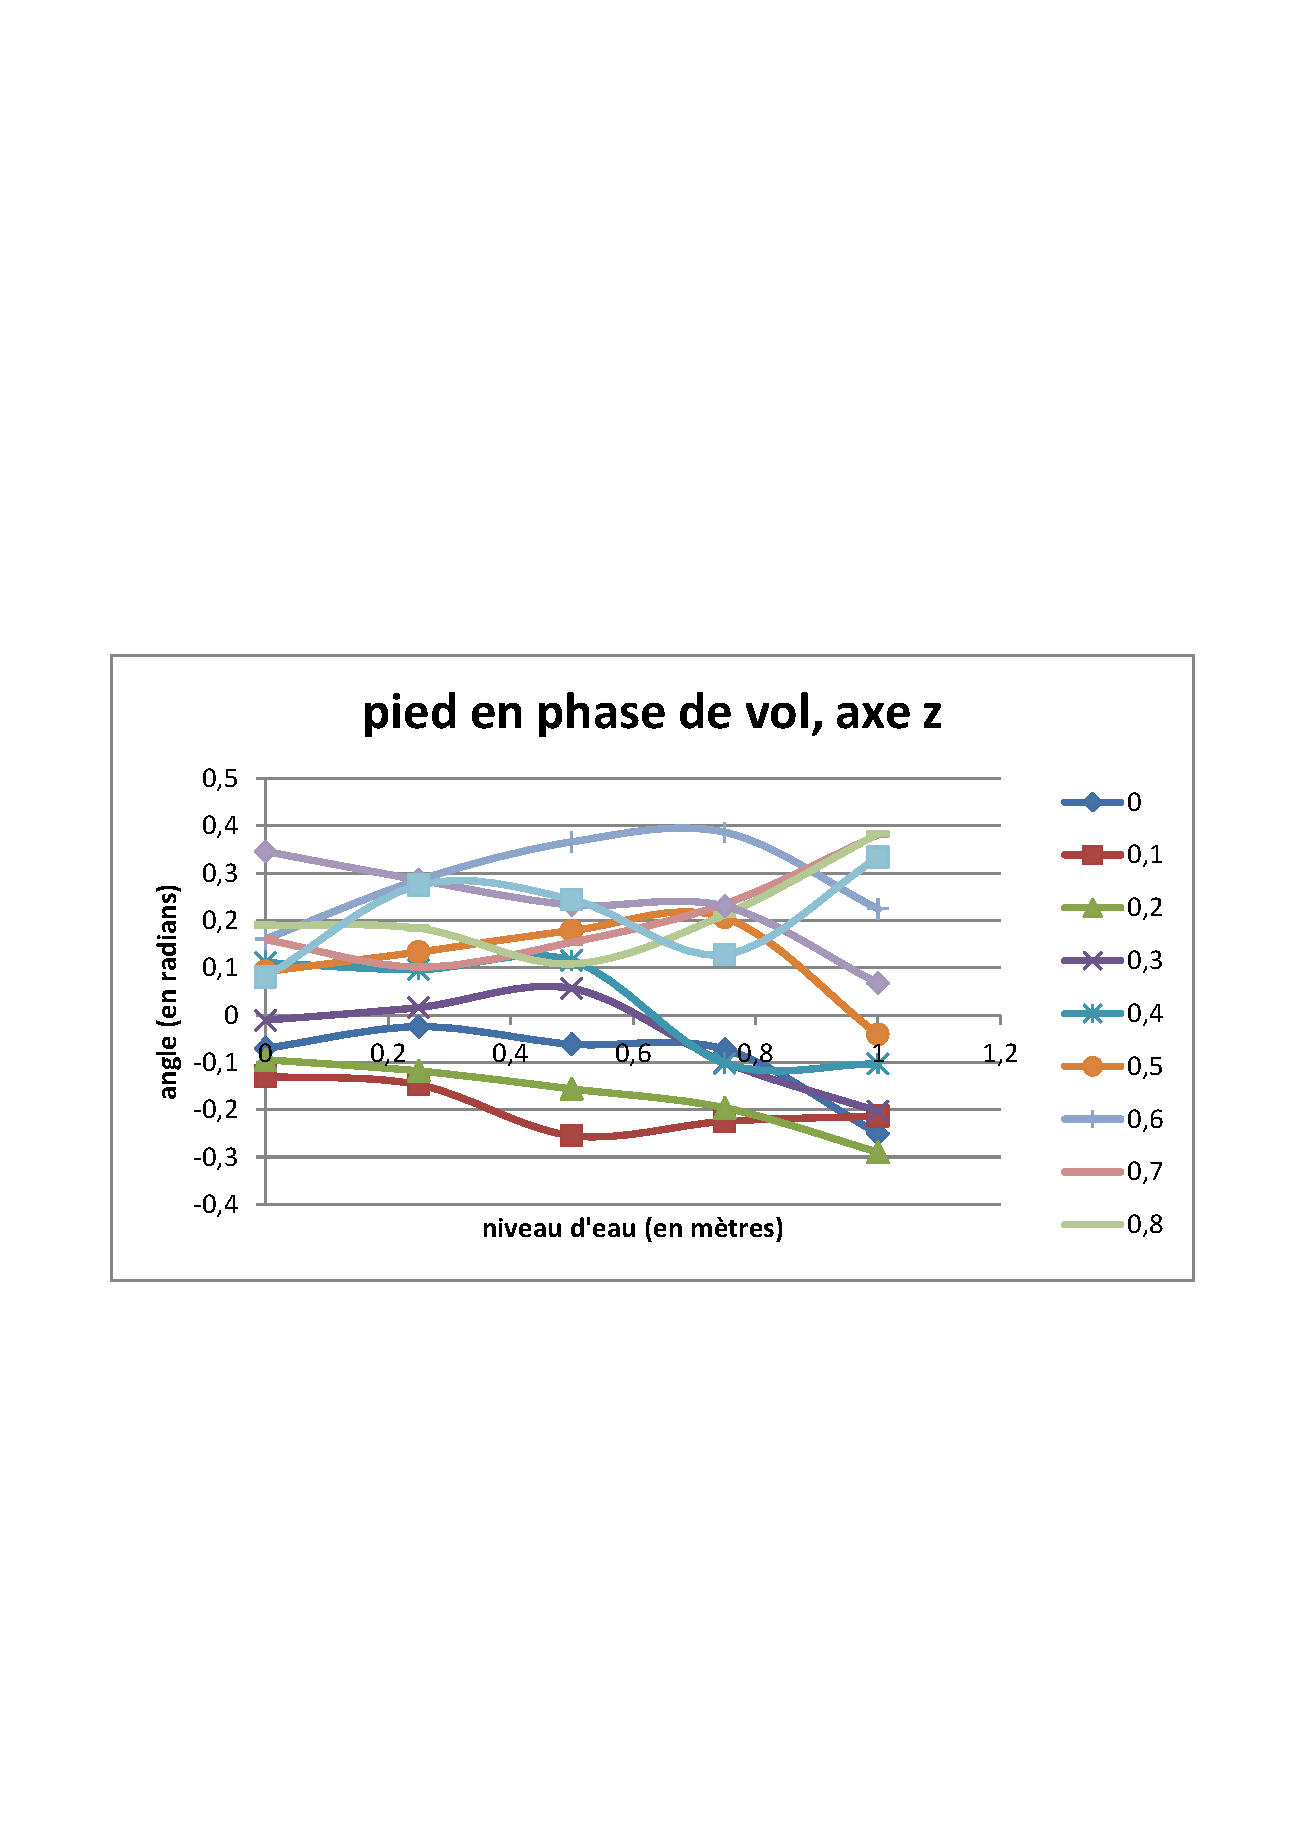
\includegraphics[scale=0.3]{traj_pts_clefs/swing_foot_z.pdf}
\caption{Trajectoires des points clefs pour les articulations concernées par l'optimisation. Chaque graphique présente en titre l'articulation et l'axe concerné.}
\label{fig:joint_space_motion_control}
\label{fig:state_machine}
\end{figure}

\end{document}
